%%%%%%%%%%%%%%%%%%%%%%%%%%%%%%%%%%%%%%%%%%%%%%%%%%%%%%%%%%%%%%%%%%%%
%% I, the copyright holder of this work, release this work into the
%% public domain. This applies worldwide. In some countries this may
%% not be legally possible; if so: I grant anyone the right to use
%% this work for any purpose, without any conditions, unless such
%% conditions are required by law.
%%%%%%%%%%%%%%%%%%%%%%%%%%%%%%%%%%%%%%%%%%%%%%%%%%%%%%%%%%%%%%%%%%%%

\documentclass[
  digital,     %% The `digital` option enables the default options for the
               %% digital version of a document. Replace with `printed`
               %% to enable the default options for the printed version
               %% of a document.
%%  color,       %% Uncomment these lines (by removing the %% at the
%%               %% beginning) to use color in the printed version of your
%%               %% document
  oneside,     %% The `oneside` option enables one-sided typesetting,
               %% which is preferred if you are only going to submit a
               %% digital version of your thesis. Replace with `twoside`
               %% for double-sided typesetting if you are planning to
               %% also print your thesis. For double-sided typesetting,
               %% use at least 120 g/m² paper to prevent show-through.
  nosansbold,  %% The `nosansbold` option prevents the use of the
               %% sans-serif type face for bold text. Replace with
               %% `sansbold` to use sans-serif type face for bold text.
  nocolorbold, %% The `nocolorbold` option disables the usage of the
               %% blue color for bold text, instead using black. Replace
               %% with `colorbold` to use blue for bold text.
  lof,         %% The `lof` option prints the List of Figures. Replace
               %% with `nolof` to hide the List of Figures.
  lot,         %% The `lot` option prints the List of Tables. Replace
               %% with `nolot` to hide the List of Tables.
]{fithesis4}
%% The following section sets up the locales used in the thesis.
\usepackage[resetfonts]{cmap} %% We need to load the T2A font encoding
\usepackage[T1,T2A]{fontenc}  %% to use the Cyrillic fonts with Russian texts.
\usepackage[
  main=english, %% By using `czech` or `slovak` as the main locale
                %% instead of `english`, you can typeset the thesis
                %% in either Czech or Slovak, respectively.
  english, german, czech, slovak %% The additional keys allow
]{babel}        %% foreign texts to be typeset as follows:
%%
%%   \begin{otherlanguage}{german}  ... \end{otherlanguage}
%%   \begin{otherlanguage}{czech}   ... \end{otherlanguage}
%%   \begin{otherlanguage}{slovak}  ... \end{otherlanguage}
%%
%%
%% The following section sets up the metadata of the thesis.
\thesissetup{
    date        = \the\year/\the\month/\the\day,
    university  = mu,
    faculty     = fi,
    type        = bc,
    department  ={Department of Computer Systems and Communications},
    author      = Jindřich Halabala,
    gender      = m,
    advisor     = {RNDr. Ondřej Krajíček},
    title       = {Experimenting with web-page structural analysis using Deep Reinforcement Learning},
    TeXtitle    = {Experimenting with web-page structural analysis using Deep Reinforcement Learning},
    keywords    = {TODO, keyword2, ...},
    TeXkeywords = {TODO, keyword2, \ldots},
    abstract    = {%

    This thesis assesses the feasibility of using deep reinforcement learning for detecting graphical user interface elements in web application screenshots. It does so by creating and training agents on environments of increasing difficulty that resemble the actual problem. Finally, it compares the resulting model with two prototypes developed using the usual approaches (traditional computer vision and deep supervised learning). We conclude that while training such a model using only reinforcement learning is possible, it does not bring many benefits for this particular problem.
    },
    thanks      = {%
      These are the acknowledgements for my thesis, which can

      span multiple paragraphs.
    },
    bib         = example.bib,
    %% Remove the following line to use the JVS 2018 faculty logo.
    facultyLogo = fithesis-fi,
}
\usepackage{makeidx}      %% The `makeidx` package contains
\makeindex                %% helper commands for index typesetting.
%% These additional packages are used within the document:
\usepackage{paralist} %% Compact list environments
\usepackage{amsmath}  %% Mathematics
\usepackage{amsthm}
\usepackage{amsfonts}
\usepackage{url}      %% Hyperlinks
\usepackage{markdown} %% Lightweight markup
\usepackage{listings} %% Source code highlighting
\usepackage{svg}      %% SVG figures
\lstset{
  basicstyle      = \ttfamily,
  identifierstyle = \color{black},
  keywordstyle    = \color{blue},
  keywordstyle    = {[2]\color{cyan}},
  keywordstyle    = {[3]\color{olive}},
  stringstyle     = \color{teal},
  commentstyle    = \itshape\color{magenta},
  breaklines      = true,
}
\usepackage{floatrow} %% Putting captions above tables
\floatsetup[table]{capposition=top}
\usepackage[babel]{csquotes} %% Context-sensitive quotation marks
\begin{document}
%% The \chapter* command can be used to produce unnumbered chapters:
\chapter*{Introduction}
%% Unlike \chapter, \chapter* does not update the headings and does not
%% enter the chapter to the table of contents. I we want correct
%% headings and a table of contents entry, we must add them manually:
\markright{\textsc{Introduction}}
\addcontentsline{toc}{chapter}{Introduction}

Certain graphical user interface (UI) testing tools, such as YSoft AIVA, interact with applications solely based on visual information. To achieve this, they must reliably detect and localize interface elements in the captured image in order to infer the UI's hierarchical structure. This process is typically carried out using traditional computer vision algorithms or deep neural networks trained via supervised learning.

This thesis investigates the experimental use of reinforcement learning (RL) algorithms for detecting user interface elements. First, a series of simulated environments with increasing complexity are created to model the problem. Next, agents are trained in these environments using various parameters and reward functions until they successfully learn to detect and localize visual elements, ranging from basic shapes to complete user interface components. This process results in an agent capable of accurately locating UI elements. Finally, the resulting approach is compared with traditional methods, focusing primarily on ease of implementation and data requirements.

The thesis is organized into five chapters. The first chapter provides a detailed overview of the problem, existing solutions, their limitations, and the rationale for using RL. The second chapter outlines the theoretical and mathematical foundations of reinforcement learning. The third chapter discusses the libraries and tools used for agent development and training. Next, the fourth chapter presents the design of simulated environments, the experiments that were conducted, and the challenges encountered. Finally, in the fifth chapter, the proposed approach is compared with traditional methods, with particular emphasis on implementation complexity and data requirements.

\chapter{User interface element detection}

YSoft AIVA\footnote{\url{https://www.ysoft.com/aiva}} is a tool for automated end-to-end testing of web applications. Unlike most competing tools, AIVA does not interact with the web page's Document Object Model (DOM). Instead, it relies entirely on visual information. This approach resembles black-box testing, as it mirrors how a real user interacts with the application, and enhances robustness in scenarios, such as when XPaths change due to newly added components. However, it introduces significant challenges, as all relevant information must be extracted from images rather than a structured markup language.

A crucial aspect of data extraction is identifying the location, size, and hierarchical relationships of all key interactive elements on a web page (e.g., buttons, icons, text fields). If performed correctly, it allows AIVA to reconstruct the DOM and localize correct elements during test execution.

This task can be addressed through either object detection or segmentation, as most objects on a web page are rectangular. However, due to the hierarchical nature of the DOM, detection is the more intuitive choice. A single pixel can belong to multiple overlapping elements, which complicates segmentation. That said, the detected information can be converted into a segmentation map if needed. This relationship is illustrated in Figure~\ref{fig:example-result}.

\begin{figure}
    \centering
    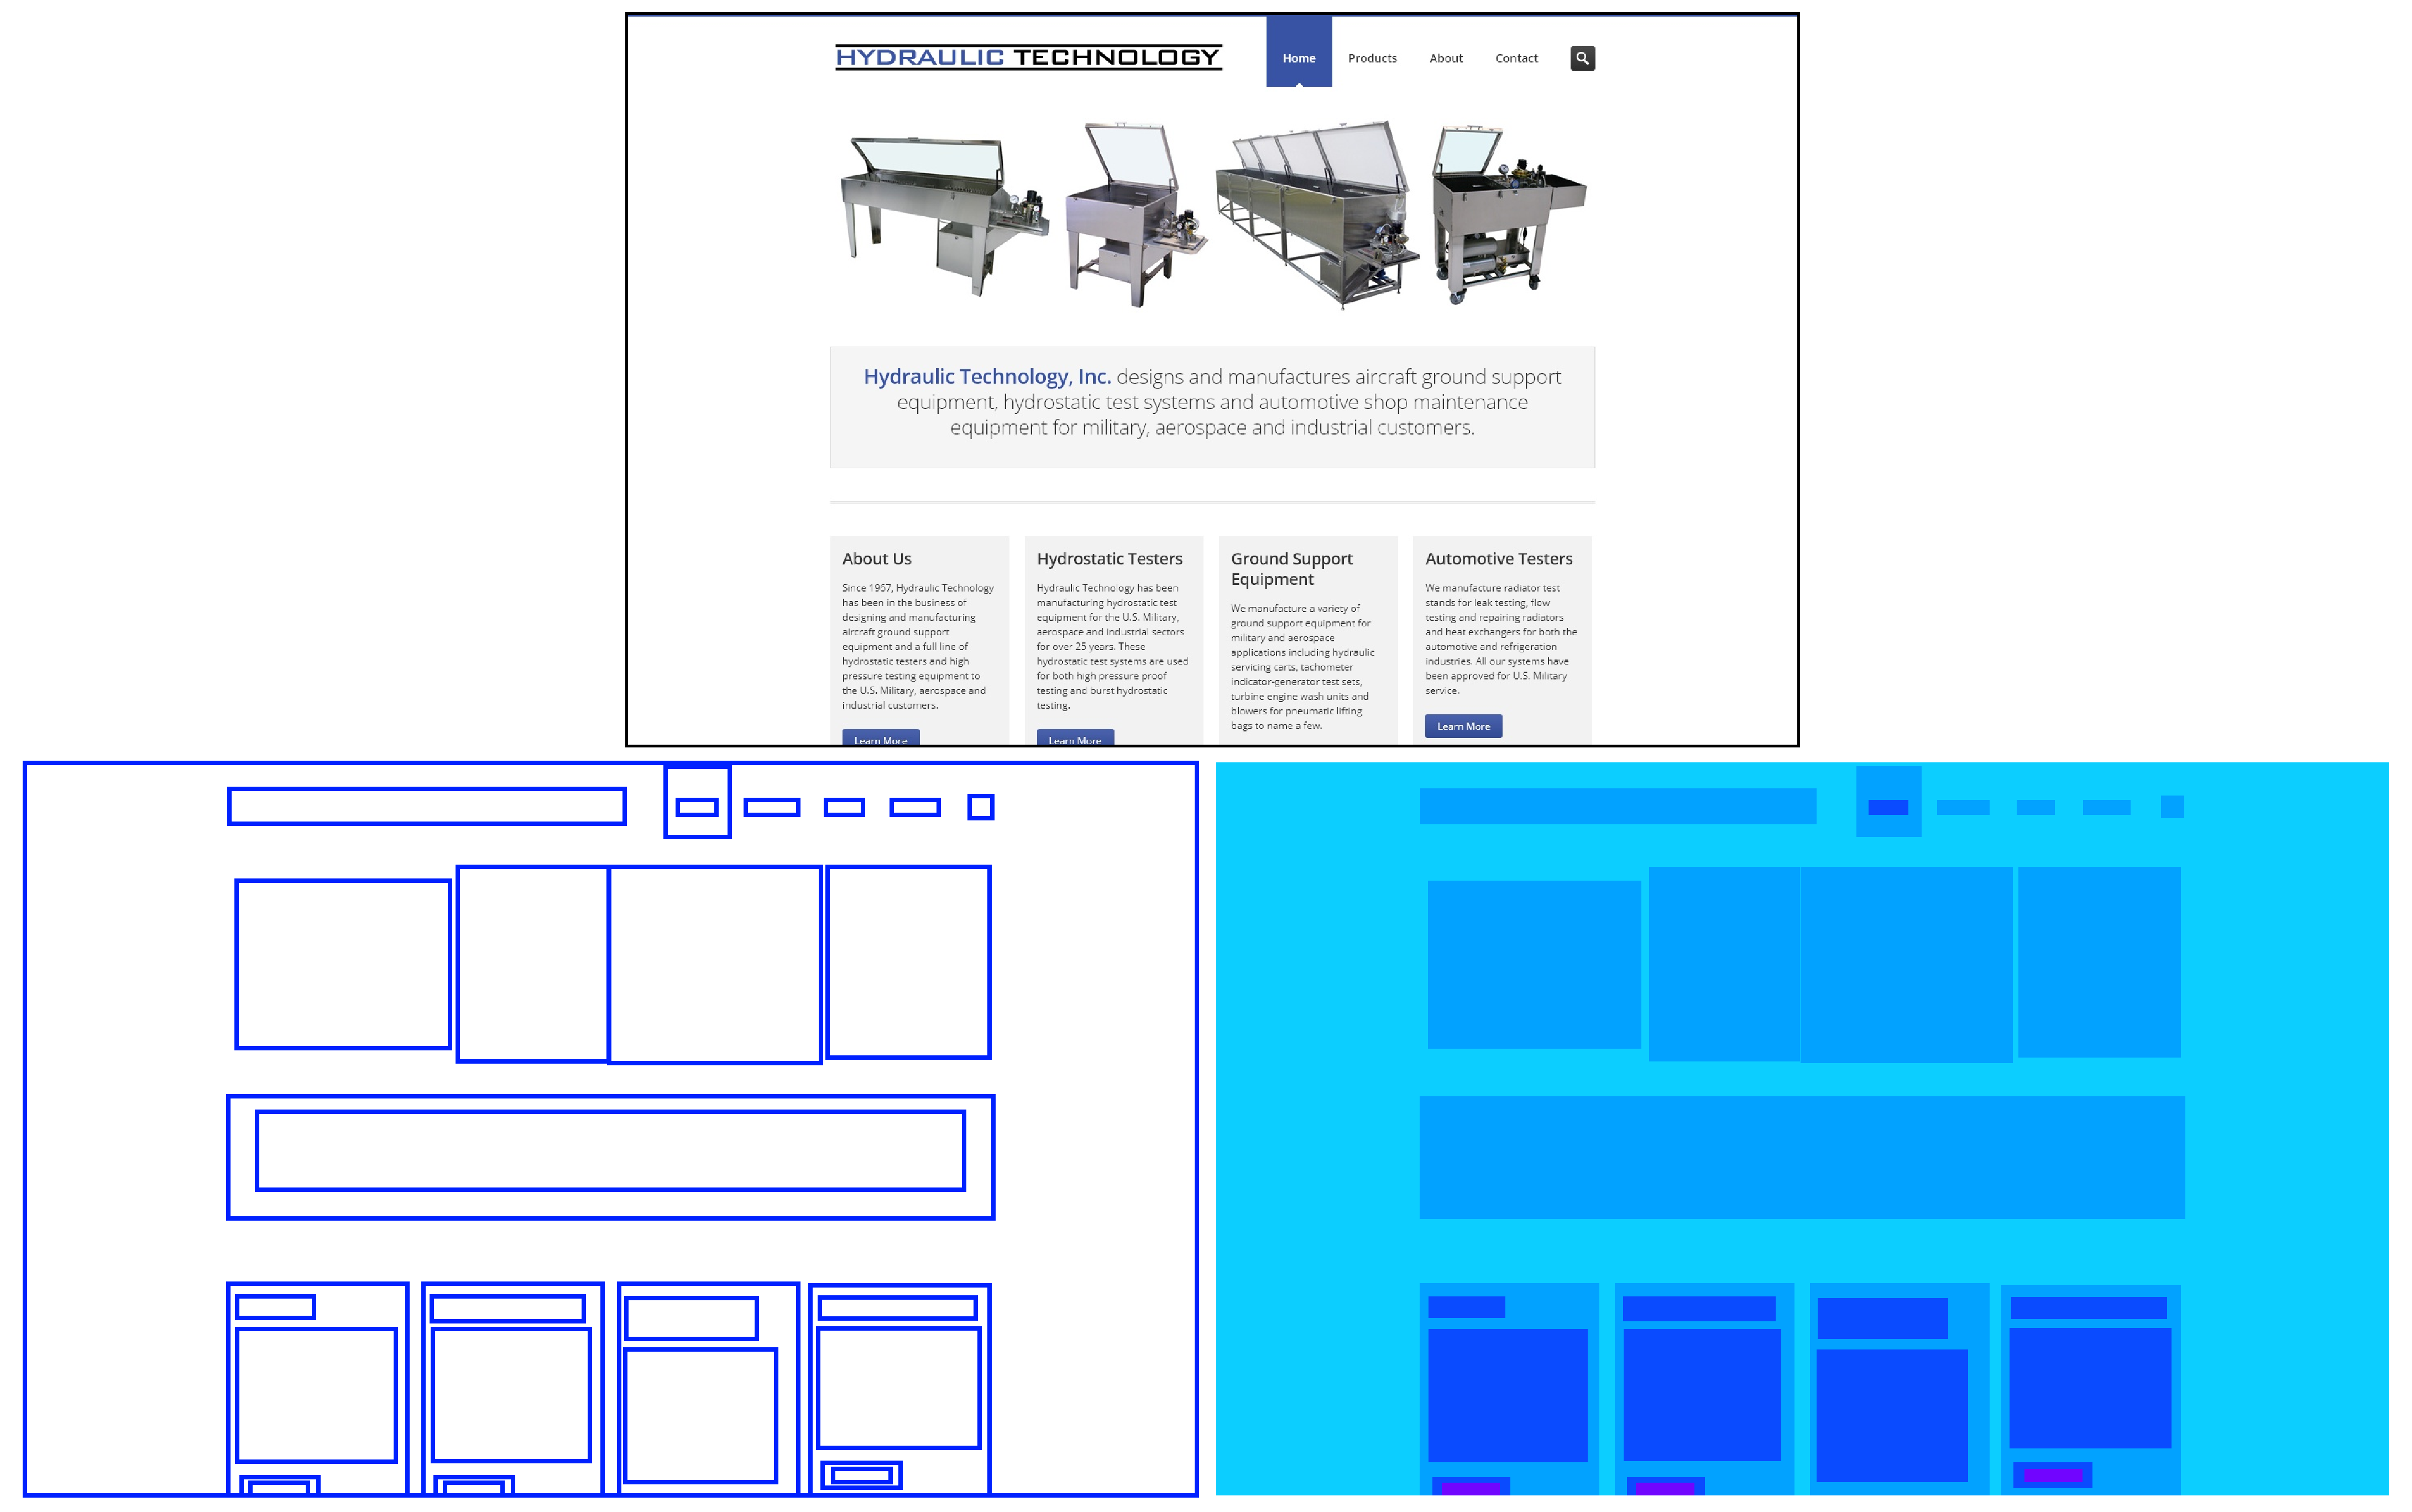
\includegraphics[width=0.7\linewidth]{diagrams/result_example.pdf}
    \caption{An example of a processed web page. The top image is the original screenshot, the middle image shows bounding boxes of detection, and the bottom image shows the same but as a segmentation map. The original screenshot comes from~\cite{aydos2020}.}
    \label{fig:example-result}
\end{figure}

Graphical user interface (GUI) object detection is usually performed using traditional computer vision (CV), deep learning-based object detection models such as R-CNNs or YOLO. A combination is also possible, for example, using a deep learning (DL) model for text and image detection and CV for the rest~\cite{ODforGUI_CV_DL_or_both}. This chapter looks at both approaches, some existing solutions based upon them, and the challenges they present. Finally, a third approach that could solve these problems is proposed based on deep reinforcement learning.

\section{Traditional computer vision-based solutions}
\label{sec:traditionalCV}

In this thesis, the term \enquote{traditional computer vision} refers to digital image processing algorithms that do not use machine learning but operate directly on pixel data. Traditional CV is challenging to use for object detection in photographs due to noise and unclear edges. However, it is well-suited for processing user interfaces. Screenshots typically lack noise (aside from occasional compression artifacts) and contain clearly defined edges

A common approach involves applying an edge detection method (e.g., Canny or Sobel), followed by post-processing steps to make the edges cleaner (e.g., morphological operations, filtering of small edges), and finally, detecting contours in the binary image. The resulting edge data are often combined with outputs from an optical character recognition (OCR) model and further processed to merge similar elements and filter out small elements that are likely just noise. This process is employed in algorithms such as REMAUI~\cite{remaui} (a tool for reverse engineering of mobile application GUIs), UISeg~\cite{uiseg} (user interface segmentation algorithm), and also in the current implementation of AIVA's element detection procedure.

Template matching represents another localization approach, though it lacks flexibility. It works reliably for highly standardized elements (e.g., checkboxes or buttons in desktop applications with a fixed GUI style). However, it is ineffective for mobile or web applications where GUI components vary widely in design~\cite{ODforGUI_CV_DL_or_both}.

Despite recent advances in deep learning, traditional CV continues to offer several advantages. It can be much more efficient and straightforward to understand, making it easier to modify and debug. Each step of the algorithm can be observed, facilitating debugging and parameter adjustment. These sorts of modifications are difficult to achieve with DL. Another significant benefit is the reduced dependency on large training datasets, which often require a lot of manual labor to create. Furthermore, this reliance increases the risk of obsolescence, as DL-based models may not generalize well to evolving GUI design trends~\cite{DLvsTCV}.

\section{Supervised deep learning-based solutions}
Over the past decade, state-of-the-art object detection algorithms have relied almost exclusively on deep neural networks incorporating convolutional layers. Two of the most prominent model families are Region-based Convolutional Neural Networks (R-CNNs) and You Only Look Once (YOLO). Generally, R-CNNs offer higher accuracy, while YOLO provides better speed, though performance varies by model and use case~\cite{ObjectDetectionHistorySurvey}.

One example of a deep learning-based GUI element detection algorithm is OmniParser\footnote{\url{https://microsoft.github.io/OmniParser/}}, a fine-tuned YOLOv8 model for parsing and labeling GUIs. It was created to enhance the performance of large multi-modal agents like GPT-4V~\cite{OmniParser}. Daneshvar et al.~\cite{GUI_YOLO_comparison} evaluated various YOLO architectures for GUI element detection, achieving promising results. During its earlier use for testing physical touchscreen devices, AIVA employed a model based on the Single Shot Detection (SSD) architecture~\cite{Horak2020thesis}.

A major advantage of DL-based approaches lies in their ability to automatically learn complex patterns from data, without requiring explicit programming or manual domain-specific tuning. However, as stated in the previous section, this reliance on a dataset is also one of the main drawbacks. Moreover, both training and inference phases typically require significantly more computational resources than traditional CV algorithms~\cite{DLvsTCV}.

\section{Object detection with reinforcement learning}

The previous two sections highlight two significant challenges. Traditional CV is insufficient for more complex images, while supervised DL methods require access to large, high-quality datasets\footnote{By \enquote{high-quality} I mean a dataset that is large, has accurate annotations, and includes larger enclosing elements. More in Subsection \ref{subsec:dataset}.}. A combination of both could, in theory, eliminate or at least mitigate these drawbacks. One possible solution involves creating a function that evaluates bounding box prediction quality based on traditional CV techniques. This function could then serve as a supervisory signal for training a deep learning model, thus eliminating the need for manually labeled ground-truth bounding boxes. Instead, only images of web applications would be required, which are significantly easier to obtain.

Supervised learning models are not applicable if we only have a numerical score for predictions rather than ground truth labels. Instead, we can use a reinforcement learning model that learns from evaluative feedback (more details on RL in Chapter~\ref{ch:dlr}).

To the best of my knowledge, no author has investigated multi-object detection using reinforcement learning. Nonetheless, prior studies have examined its use for single-object detection in photographs~\cite{iterative_od_with_rl, hierarchical_od_with_drl} and for region proposal in multi-object detection~\cite{drl_rpn}. They all use ground-truth labels for learning since creating a CV-based reward function for photographs would be very difficult. However, for GUI environments, such an approach may be feasible.

\chapter{Deep reinforcement learning}
\label{ch:dlr}

The theory behind reinforcement learning is essential for understanding the terminology and decisions presented in the following chapters. This chapter provides the necessary background to understand the remainder of this thesis. Note that this is a brief, non-exhaustive introduction covering only the most important algorithms and definitions.

Unless stated otherwise, the notation and information used in this chapter are adopted from \textit{Grokking Deep Reinforcement Learning} by Miguel Morales~\cite{GDRL}.

\section{Machine learning}
Machine learning (ML) is the study of algorithms that allow computers to learn from data without explicit programming. It is often split into three main categories: supervised learning, unsupervised learning, and reinforcement learning\footnote{Other categories, such as semi-supervised or self-supervised learning, are also sometimes stated, but these are generally considered modifications or combinations of the three primary categories.}~\cite{IB031}.

In supervised learning (SL), the goal is to make predictions based on labeled data available during training, such as in classification or regression tasks. In unsupervised learning (UL), no correct labels are known, so it is more about finding patterns in the provided data. This approach can be used to, for example, separate the data into groups (clustering) or to generate new, similar data using models such as autoencoders or generative adversarial networks~\cite{IB031, PV021}.

Similar to SL, reinforcement learning involves learning a mapping from inputs to outputs, but differs fundamentally in the type of feedback provided. Unlike in SL, where the correct labels are provided for training purposes, RL relies only on the feedback from a reward function. This function evaluates the agent's decisions based on their outcomes, by providing scalar feedback that reflects the quality of the chosen actions. The agent aims to learn to make decisions that maximize this reward through trial and error. RL is ideal for decision-making, especially in environments where the optimal strategy is unknown or difficult to obtain.

\section{Reinforcement learning}
Reinforcement learning problems consist of two interacting entities: the agent and the environment. The agent is the algorithm taught to make decisions. The environment comprises everything external to the agent. For example, in a driving task, the environment includes other vehicles, road conditions, pedestrians, and the controlled car itself.

The typical interaction between agent and environment in RL follows a cycle, as illustrated in Figure \ref{fig:rl-cycle}. In the beginning, the environment is in some initial state. The agent observes the state (although in many cases, it may only have access to a partial observation of the full state) and chooses an action it thinks is the best. The environment receives and reacts to this choice, changing its inner state. The agent observes this new state and gets rewarded based on the chosen action. The agent can then update its behavior based on this feedback. Then, it again chooses an action, and the cycle repeats.

\begin{figure}
    \centering
    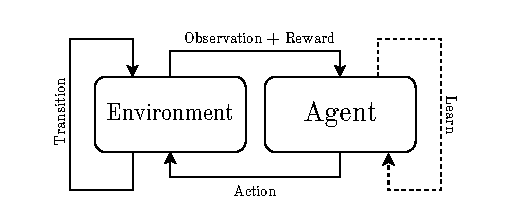
\includegraphics[width=1\linewidth]{diagrams/rl_cycle.pdf}
    \caption{The reinforcement learning cycle}
    \label{fig:rl-cycle}
\end{figure}

A single iteration of this cycle is referred to as a time step and generates an experience -- a tuple of the original state $s$, the action taken $a$, the reward given $r$, and the new state $s'$. Depending on the task, the cycle may continue indefinitely or terminate once the environment reaches a designated terminal state. For example, in a chess game, the end is defined as winning, losing, or a draw. Such tasks are called episodic, with all experiences from the initial to the terminal state forming an episode. If there is no well-defined end, the task is referred to as continuous.

The reward function may be dense, sparse, or lie somewhere in between. A dense reward function awards the agent a non-zero reward in each iteration of the RL cycle. A sparse reward function only gives a non-zero reward when the environment transitions into a terminal state. While dense reward functions are generally easier to learn from, in some cases, they can be challenging to implement. In the chess example, we know that losing is negative and winning is positive, but judging a single move is problematic unless we know the optimal strategy.

Reinforcement learning is challenging due to the sequential, evaluative, and sampled feedback.

The sequentiality comes from the fact that most tasks span multiple time steps. The consequences of an action might not be immediately apparent. When an episode ends with a very negative result, it can be difficult to determine which of the preceding actions is the cause, as it is often not the last action taken.

Evaluative feedback refers to the reward being provided as a scalar value. Without additional context, it is impossible to know if the received reward was the best possible and if we should thus repeat the decision in similar states or whether it was terrible and should be avoided in the future. This issue leads to the need for exploration discussed in Section~\ref{sec:eplor-exploit}.

The agent can only learn from the states it has visited and the actions it has taken, thus the feedback it gets is sampled. In many real-life RL problems, there are so many states that trying every combination of state and action is impossible. This challenge also exists in supervised learning, as the dataset will never contain all the data we might encounter. However, in reinforcement learning, this is even worse as the agent must collect all the data on its own.

\section{Markov decision process}
In order to define RL and its objective, it is first necessary to define the environment. There are multiple ways to do so, but the most common representation is a Markov decision process (MDP). An MDP is defined as a tuple $(S, A, p, r)$.

$S$ is the state space, a set of all possible environment states. It can contain both discrete and continuous values. At each time step $t$, the MDP is in a state $s_t\in S$.

$A$ is the action space, a set of all possible actions an agent can perform in this MDP. It may also be discrete, continuous, or a combination of both. At each time step $t$, the agent chooses an action $a_t\in A$ based on the observed state $s_t$.

$p$ is the probabilistic transition function $p\colon S \times A \to \mathcal{D}(S)$. For a given state $s\in S$ and a given action $a\in A$, it returns a probability distribution over the states $s'\in S$. It tells us the probability of the MDP transitioning from the state $s$ to a state $s'$ given that an action $a$ was selected. Formally, it is defined as:
\begin{equation}
p(s' \mid s,a)=P(S_t=s'\mid S_{t-1}=s,A_{t-1}=a)    
\end{equation}
The sum of all transition probabilities for each individual state-action pair must equal one:
\begin{equation}
\sum_{s'\in S} p(s'\mid s,a)=1, \forall s \in S, \forall a \in A
\end{equation}

If the environment does not allow for some action $a^{\times}$ to be performed in a state $s$, we define a degenerate transition distribution for that state-action pair:
\begin{equation}
    p(s'\mid s, a^{\times}) =\begin{cases}1 & s' = s\\0 & \text{otherwise} \end{cases} 
\end{equation}

Lastly, $r$ is the reward function. Depending on the use case, it can be defined either as $r\colon S \times A \to \mathbb{R}$ \cite{PA230} -- the expected reward for choosing an action $a$ in a state $s$:
\begin{equation}
r(s,a)= \mathbb{E} [R_t\mid S_{t-1}=s, A_{t-1}=a]
\end{equation}
or as $r\colon S\times A \times S \to \mathbb{R}$ -- the expected reward for choosing an action $a$ in a state $s$ given we transition into a state $s'$:
\begin{equation}
r(s, a, s')= \mathbb{E} [R_t\mid S_{t-1}=s, A_{t-1}=a, S_t=s']
\end{equation}

Another property often defined is the set of initial states $S^i \subseteq S$. When an MDP is initialized, the initial state is chosen from this subset using a probability distribution $\mathcal{I}$ over these states.

Similarly, a set of all terminal states may be defined. The MDP terminates when it transitions into one of the terminal states. Alternatively, the explicit definition of terminal states can be omitted by modeling them as absorbing states. This involves defining the transition function such that any action taken in a terminal state leads back to that same state with a probability of 1, and ensuring the reward for such transitions is 0.

Simple Markov decision processes can be visualized as diagrams, as illustrated in Figure \ref{fig:mdp}.

\begin{figure}
    \centering
    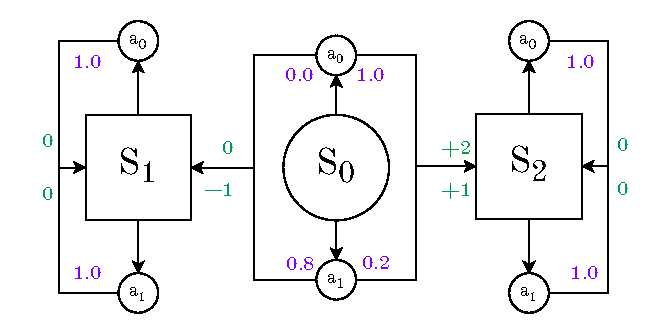
\includegraphics[width=1\linewidth]{diagrams/mdp.pdf}
    \caption{An example of a graphical representation of a Markov decision process. Squares depict terminal states. Transition probabilities (purple) and rewards (green) are indicated.}
    \label{fig:mdp}
\end{figure}

\subsection{Markov property}
\label{subsec:markov_property}
The probabilistic transition function $p$ only takes the current state and action as inputs. Importantly, it does not consider history. The probability of transitioning from a state $s$ to a state $s'$ under an action $a$ depends only on $s$ and $a$, not on how the MDP arrived at $s$. This memorylessness of MDPs is known as the Markov property. It is important to remember when implementing an environment since many RL algorithms rely on the environment to satisfy the Markov property. It can be formally defined as
\begin{equation}
P(S_{t+1}\mid S_t,A_t)=P(S_{t+1}\mid S_t,A_t,S_{t-1},A_{t-1}, \dotsc)
\end{equation}
An example of an environment that violates this property could be the game of Pong\footnote{\url{https://en.wikipedia.org/wiki/Pong}}, where the state is only the current frame. From just one frame, it is impossible to know in which direction or at what speed the ball will move after the next action. This problem can, of course, be resolved by including the position, speed, and direction of the ball's movement in the state (or using other techniques such as frame-stacking, where multiple preceding frames are included in the observation). In real-world scenarios, fully capturing movement may require including higher-order dynamics like acceleration or jerk.

\subsection{Partially observable MDPs}
Regular MDPs can be somewhat limiting when modeling real-life scenarios, but many modifications exist that address some of the issues. In RL, we often encounter partially observable MDPs (POMDPs) where the agent does not have access to the true state but only an observation of it. POMDPs further define the observation space $\mathcal{O}$ and a state-observation mapping function $\epsilon \colon S \to \mathcal{D}(\mathcal{O})$.

\section{Policy}
Now that the environment is formally defined using an MDP, we can also formally define the agent. We can imagine the agent as some entity that receives a state $s$ (or an observation of it) and, based on it, chooses an action $a$ that is then performed, and the agent receives a reward $r$ and a new state $s'$. As mentioned, we call the tuple $(s, a, r, s')$ an experience. The entire chain of these experiences is called a trajectory $\tau$. Since the ending state of one experience and the initial state of the following experience is the same, it can be simplified to: $s_0,a_0,r_1,s_1,a_1,r_2,\dotsc \in (S\times A \times \mathbb{R})^{*}$. Note that a trajectory is infinitely long since even in a terminal state, we can still perform an action; it just gives zero reward and never transitions the environment into a new state. History is then some prefix of a trajectory ending in a state: $s_0,a_0,r_1,s_1,a_1,r_2,\dotsc, a_{t-1},r_t,s_t\in (S\times A \times \mathbb{R})^{*}\times S$. The agent makes the decisions based on some rules. We call policy $\pi$ a function $\pi\colon (S\times A \times \mathbb{R})^{*}\times S \to \mathcal{D}(A)$, which returns a probability distribution over the action space based on the history up to that point~\cite[p. 19]{PA230}.

If the Markov property is fulfilled, we can simplify policy to just $\pi\colon S \to \mathcal{D}(A)$ because, in that case, the environment is memoryless, and thus, it does not matter how it ended up in the state $s_t$. Thanks to this, the agent (and its underlying policy) can also be memoryless. Note that this is only true if the agent receives the entire state, so this simplification can not be applied to POMDPs (two different states might produce the same observation, and the history might be helpful to differentiate between them).

We can further simplify the policy by making it deterministic -- instead of returning a probability distribution $\mathcal{D}(A)$ it returns just a single action $a$. Such policy can be defined as just $\pi\colon S \to A$.

\section{The goal of RL}
\label{sec:goal}
Now that we have fully formally defined the environment (MDP) and the agent (policy), we can define the goal of RL. The goal is to find a policy $\pi^*$ that maximizes the expected discounted cumulative reward, also called the discounted return. The cumulative reward (or return) of a trajectory $\tau$ is defined as the sum of all received rewards:
\begin{equation}
G(\tau) = r_1+r_2+r_3+\dotsb = \sum_{i=0}^{\infty} r_{i+1}
\end{equation}
To get the discounted return, we exponentially decay the rewards by some discount factor $\gamma \in [0,1]$. The discounting has two reasons. Since the trajectory can be infinitely long, if the policy found a cycle with a positive reward (even very small), it would lead to the cumulative reward being infinite. Second, it encourages policies that not only reach the maximum reward but also get it as fast as possible because the reward will be less discounted. So, the discounted return $G$ on a trajectory $\tau$ with discount factor $\gamma$ is defined as:
\begin{equation}
G(\tau)=r_1+\gamma \cdot r_2+ \gamma^2 \cdot r_3+\dotsb = \sum_{i=0}^{\infty} \gamma^i\cdot r_{i+1}
\end{equation}
Finally, the expected discounted cumulative reward. As stated before, the environments are often stochastic. They can start in many different states (with possibly different probabilities), and taking an action in a state can lead to different transitions (again with possibly different probabilities). Because of this, even a deterministic policy can have different trajectories on the same MDP each time, and those can, in turn, have different returns. Thus, it is important to find such a policy that will, on average, have the highest discounted return, not just in some specific single case.

\section{Value functions}

For a given policy $\pi$, we can calculate its value functions. These are functions that describe how this policy performs in some given environment. They can be used to compare policies or for learning purposes (see Subsection \ref{subsec:value-based-methods}).

\subsection{State-value function}
\label{subsec:state_value_func}
The state-value function $v_\pi\colon S\to \mathbb{R}$ (often called just the value function) tells us the expected return of policy $\pi$ when starting in a state $s$.
\begin{equation}
v_\pi(s) = \mathbb{E}_\pi [G_t\mid S_t=s]
\end{equation}

If we know the underlying MDP, we can calculate it directly using the Bellman equation:

\begin{equation}
v_\pi(s) = \sum_a \pi(a\mid s) \cdot \sum_{s',r} p(s',r\mid s,a)\cdot[r+\gamma v_\pi(s')], \forall s \in S
\end{equation}

Due to the recursive nature of this formula, it would be difficult to calculate directly, so in practice, an iterative algorithm that uses an already existing approximation for the next state is used (often called policy evaluation). When we cannot access the MDP, we can use algorithms such as Monte Carlo or Temporal difference that repeatedly interact with the environment to collect experiences and then use this data to approximate the value functions.

\subsection{Action-value function}

Knowing how well the policy performs in a state can be useful, but it does not help it decide which action to take (unless it also has access to the transition function). The action-value function $q_\pi\colon S \times A \to \mathbb{R}$ tells us the expected return of policy $\pi$ if the agent were to select action $a$ in state $s$ and then follow the policy until it reaches a terminal state.

\begin{equation}
q_\pi(s,a) = \mathbb{E}_\pi [G_t\mid S_t=s,A_t=a]
\end{equation}

Knowing the action-value function can help us improve the policy. Algorithms, such as Q-learning and DQN, are based on this principle.

\subsection{Action-advantage function}

Lastly, the advantage function $a_\pi$ is a modification of the action-value function that tells us how much better (or worse) it is to take an action $a$ in a state $s$ compared to following the policy:

\begin{equation}
a_\pi(s,a) = q_\pi(s,a)-v_\pi(s)
\end{equation}

When using a neural network as the approximator, it is common to approximate state-value and advantage-value functions separately and combine the results instead of directly approximating the action-value function (this technique is known as the dueling network architecture and was introduced in \cite{dueling_arch}).

\section{Exploration-exploitation tradeoff}
\label{sec:eplor-exploit}
As mentioned in Subsection \ref{subsec:state_value_func}, many RL algorithms rely on approximating a value function using an iterative algorithm and then use this information to improve the policy. They must repeatedly interact with the environment and collect experiences to make the approximation. To create the best approximation, it would be best to run the policy from every possible state and try every possible action, ideally many times, to account for randomness. Obviously, this is not feasible for any environments with more than a few thousand states, and it is impossible for environments with continuous state or action spaces.

Since exhaustive exploration is infeasible, RL algorithms must balance two competing objectives: discovering new strategies (exploration) and leveraging known good strategies (exploitation). This challenge is known as the exploration-exploitation tradeoff. Should we rather try new actions and risk wasting time on unproductive paths (explore), or stick to what we know works reasonably well, but risk completely missing some better strategies (exploit)? To measure how much of the training was \enquote{wasted} on exploring, we can use a metric called regret. To calculate regret $R$ at time $T$, we sum the differences between the expected reward for the optimal action and the actual reward for the selected action for every step.

\begin{equation}
R(T) = \sum_{t=1}^{T}(\mathbb{E}[r^*]-r_t)
\end{equation}

Note that the optimal strategy must be known to calculate the expected optimal reward ($\mathbb{E}[r^*]$). If it is not known, other strategies must be used.

The goal is to find the optimal policy while maintaining the lowest total regret. To manage this tradeoff effectively, various exploration strategies have been developed. Below are three commonly used approaches:

\begin{itemize}
    \item (Decaying) epsilon-greedy exploration strategy -- given some constant $\varepsilon \in [0,1]$, choose a random action with the probability of $\varepsilon$; otherwise, choose the action currently estimated to be the best. More commonly, $\varepsilon$ is not a constant; instead, it gets lowered (decayed) as training progresses.
    \item Upper confidence bound strategy -- when choosing which action to take next, a bonus is added to the estimates with lower confidences (those that are less explored). The bonus is calculated as $c\sqrt{\frac{\ln{t}}{N_t(a)+1}}$ where $c$ is some constant describing the importance of this bonus, $t$ is the episode number and $N_t(a)$ is how many times the action $a$ was already chosen (plus one to avoid division by zero).
    \item Softmax exploration strategy -- the chance of selecting a certain action is proportional to its action value estimate. To get the probabilities, we pass the estimates through the softmax function, which will normalize them so that they are all between zero and one and their sum is equal to one. The softmax function is defined as $\sigma (v)_i = \frac{e^{v_i}}{\sum^{K}_{j=1}e^{v_j}}$ for the $i$-th value of a vector $v$ with $K$ elements. This strategy would not work very well at the beginning when the estimates have high variance, so we also divided the estimates by a decaying hyper-parameter $\tau$ called temperature, which makes it so the estimates are less important at the beginning of the training.
\end{itemize}



\section{Reinforcement learning algorithms}
\label{sec:algos}

Especially in recent years, many reinforcement learning algorithms have been published. The following subsections only describe the three main categories with a couple of examples, as detailed descriptions of individual algorithms are not required to understand the following chapters.

\subsection{Value-based methods}
\label{subsec:value-based-methods}

The most straightforward approach to reinforcement learning is learning to approximate the action-value function (either directly or calculating it using the state-value and advantage-value functions) and then using a greedy policy that selects the best action based on these approximations.

For simple environments with small discrete state and action spaces, it is possible to have a table of every state-action combination (tabular algorithms). There are many different algorithms utilizing this principle. They differ in the way they calculate the approximations (Temporal difference (TD), Monte-Carlo (MC), $\lambda$-TD), whether they use the same model for the approximation and exploration (SARSA, Q-learning), and in their exploration strategies. Some more advanced algorithms approximate not only the Q function but also the underlying MDP to learn more efficiently (Dyna-Q).

While tabular algorithms can work very well for simple environments, they are unusable for any more complex ones. Even for just a $100 \times 100$ pixel binary image state, a table of over $10^{3011}$ numbers would be necessary.

Deep learning is utilized for these more complex environments. The approximator is a neural network whose loss function is calculated as the difference between the approximations and actual values gathered during exploration. These methods often use a replay buffer -- a data structure that collects experience tuples from previous runs. When learning, examples are picked randomly from this buffer, reducing the bias in data caused by the experiences from one episode not being independent. These methods include algorithms such as Neural Fitted Q-iteration (NFQ), Deep Q-Learning (DQN), and Double DQN (DDQN).

\subsection{Policy-based methods}

While value-based methods create policies indirectly based on a value function, policy-based methods learn the policy directly by outputting a probability distribution over actions. The learning is usually done by maximizing the probability of taking actions with a bigger advantage estimation using gradient ascent.

Purely policy-based algorithms are rarely used nowadays, but they are an important part of the actor-critic architecture introduced in the following subsection. Policy-based algorithms include REINFORCE and Vanilla Policy Gradient (VPG).

\subsection{Actor-critic methods}

Actor-critic methods combine both value-based and policy-based methods into one. They are composed of two parts: the actor and the critic. The critic is a value function estimator of the actor, which represents the policy by choosing the actions. The critic learns just like the value-based methods by minimizing TD or MC errors. The actor then learns by maximizing the expected return based on the value estimations provided by the critic.

Actor-critic methods combine the strengths of both value-based and policy-based methods. They are more stable, sample efficient, and can deal with discrete and continuous action spaces. State-of-the-art actor-critic algorithms include Twin Delayed Deep Deterministic Policy Gradient (TD3), Soft Actor-Critic (SAC), and Proximal Policy Optimization (PPO).

\chapter{RL in practice}

The previous chapter briefly explained the theory and terminology behind RL. This chapter follows up with an introduction to RL libraries and their usage. It should give enough context to make the source code of the experiments done in this thesis understandable.

As with most machine learning tasks, Python is one of the most popular programming languages for RL, so I decided to use it in this thesis. AIVA is written mainly in .NET, but this should not be a problem since most machine learning libraries allow export into a standard format such as ONNX\footnote{\url{https://onnx.ai/}} so that agents trained in Python can also be run natively in other programming languages.

\section{Gymnasium}
\label{sec:gym}
Gymnasium\footnote{\url{https://gymnasium.farama.org/}} is a Python library that allows for easy creation of RL environments. It is a maintained fork of the Gym\footnote{\url{https://www.gymlibrary.dev/}} library developed by OpenAI. Its primary purpose is to define a unified environment API. However, it also contains many wrappers that simplify processes such as normalization, clipping, training recording, or vectorization of parallel training. It also provides many predefined environments that can be used to test new RL algorithms. The information in this section comes from the official Gymnasium documentation~\cite{gym-docs}.

An environment is a Python class that inherits from the \texttt{Env} class. Inside the initialization method of this class, the observation and action space types must be defined. Gymnasium provides the following types of spaces:

\begin{itemize}
    \item \texttt{Box} -- represents a tensor ($n$-dimensional matrix of numbers) of a fixed shape. The numbers inside can be both bounded and unbounded. This type is useful for a representation of images or continuous actions.
    \item \texttt{Discrete} -- represents a space of finitely many integers. It is useful for representing discrete action spaces.
    \item \texttt{MultiBinary} -- tensor of boolean values.
    \item \texttt{MultiDiscrete} -- tensor of discrete values. 
    \item \texttt{Text} -- a string composed of specified characters.
    \item Composite spaces -- multiple fundamental spaces can be combined into a \texttt{Dictionary}, \texttt{Tuple}, \texttt{Sequence} of variable length, a \texttt{Graph} or a \texttt{Union}.
\end{itemize}

The environment class also requires the following methods to be implemented:

\begin{itemize}
    \item \texttt{reset} -- called to begin a new episode. It resets the environment to an initial state and returns the initial observation and a dictionary with auxiliary information for debugging or other purposes. It takes a seed value as an optional parameter.
    \item \texttt{step} -- performs a single time step of the environment. Its only input is the action to be performed, which has to adhere to the type defined in the initialization method. It transitions the environment to a new state, returning the new observation, the reward awarded for taking the action, whether the reached state was terminal, whether the episode was truncated (e.g., due to reaching a time limit), and again, a dictionary with auxiliary information.
    \item \texttt{render} -- a method for getting the current state of the environment in a human-friendly format. Each environment can define multiple render modes, one of which can be selected during initialization. Most common formats include an RGB frame, text, or a list of RGB frames. This method can be either called manually by a user or, more often, by a monitoring wrapper of the environment.
    \item \texttt{close} -- a clean-up method. Should close render windows, end database connections, etc.
\end{itemize}

Once an environment is defined, it should be registered using the \texttt{gymnasium.envs.registration.register} function, which allows it to be later created using the \texttt{gymnasium.make} function. Such an environment can then be wrapped in the aforementioned wrappers and passed to a RL algorithm.

\section{Stable-Baselines3}
Stable-Baselines3\footnote{\url{https://stable-baselines3.readthedocs.io/en/master/}} (SB3) is a Python library containing implementations of RL algorithms. It originated as a maintained fork of the OpenAI Baselines\footnote{\url{https://github.com/openai/baselines}} library but has since evolved to include numerous additional algorithms, an improved API, and comprehensive documentation. The algorithms are implemented using PyTorch, allowing simple modifications of the underlying neural networks and GPU-accelerated training. These algorithms interact with environments defined using the Gymnasium API described in Section~\ref{sec:gym}. The information in this section is from the official SB3 documentation~\cite{SB3-docs}.

To create a new model, one instantiates a class provided by SB3 (such as \texttt{PPO}, \texttt{A2C}, or \texttt{DDPG}) and supplies the environment along with additional parameters, including hyperparameters, GPU selection, and logging options. The library also supports saving and loading models via the \texttt{save} and \texttt{load} methods.

Once a model has been created, it can be trained using the \texttt{learn} method, which trains the model for the provided amount of time steps. Additionally, a callback can be passed as well. Callbacks are special classes that can call functions when certain events happen during training. For example, the \texttt{EvalCallback} evaluates the model every $n$ episode and can additionally save the model on the new best mean reward. SB3 also provides an API for creating custom callbacks.

Inference on a model is done through the \texttt{predict} method, which returns the model's decided action for a given observation.

I chose this library over others mainly because it contains algorithm implementations, simple-to-use API, and good documentation. I chose not to implement the algorithms on my own since they would probably perform worse, and it is unlikely that these implementations would change the outcome of this thesis.

\section{Optuna}
\label{sec:optuna}

Optuna\footnote{\url{https://optuna.org/}} is an open-source framework used for automated hyperparameter search (or, in general, for optimizing any function with parameters). It uses state-of-the-art algorithms to suggest hyperparameters based on previous experiences, making it much more time-efficient than usual methods such as grid search. Once again, the information in this section is sourced from its official documentation~\cite{optuna-docs}.

Optuna can optimize any objective function. Such function takes a \texttt{trial} object as an input, uses its methods like \texttt{trial.suggest\_int} or \texttt{trial.suggest\_categorical} to get the suggested hyperparameters and returns a float representing how well the objective was met (this is most often some accuracy metric, in the case of RL, it is the mean episode reward). A study is then created using the \texttt{optuna.create\_study} function. This study can then be optimized for a number of trials, after which it returns the hyperparameters that were found to be the best.

A study can be connected to a relational database that stores previous trials. The results can then be visualized using Optuna Dashboard\footnote{\url{https://optuna-dashboard.readthedocs.io/}}. It plots information such as hyperparameter importance, the tuning progression, and much more.

It is also possible to run multiple Optuna instances in parallel using the same database. This allows for effortless distributed tuning on multiple machines with almost linear scaling.

Optuna can also be configured to prune attempts unlikely to beat the current best attempt if the objective function can produce intermediate values. This change can speed up the process significantly.

\section{Hardware}

Most state-of-the-art RL algorithms are based on deep learning. Powerful enough hardware is needed to train large neural networks in a reasonable time. Most of the experiments in this thesis were done on my personal computer (Intel i5-12400, NVIDIA RTX 3080). For long-running experiments, I used one of Y Soft's GPU nodes (AMD Ryzen 9 5950X, NVIDIA RTX A4000). The speed of these two machines is very comparable in a single environment, but the 16 cores of the AMD Ryzen 9 5950X significantly outperform the Intel i5-12400's six cores in vectorized environments.

\chapter{Experiments}
\label{ch:experiments}

\section{Defining the problem}
\label{sec:problem_definition}

Before we start training models, we must define the problem we are trying to solve. The goal is to create an algorithm that receives an image as input (be it directly a screenshot of a website or some preprocessed version to simplify the task). It outputs a set of bounding boxes, each of which is the bounding rectangle of an object in the image. The algorithm should find all objects in the image.

With regular supervised learning, the variable length of the output could be a challenge. Each image can contain a different amount of objects. Thankfully, this is not an issue for RL, as it is naturally sequential with different episode lengths. We need the agent to perform such actions that are convertible into bounding boxes (be it a one-to-one relationship where each action is one selection or a many-to-one relationship where multiple actions combined create a selection). Already found objects have to be marked somehow since the agent has no memory (see Subsection \ref{subsec:markov_property}).

First, we have to decide on the state and action spaces and the representation of the states and actions. The input image can be used directly as the state. More formally, the input type will be represented by a tensor of size $C\times M \times N$ where $C$ is the channel count (3 for RGB images, 1 for grayscale and binary images), $M$ and $N$ are the width and height of the image. The values of this tensor are integers in the range 0-255 or real numbers in the range 0-1 after normalization. The \texttt{Box} Gymnasium type is ideal for this representation. In theory, the \texttt{MultiDiscrete} could be more suitable as the values are discrete, not continuous, but SB3 does not currently support using convolutional layers on discrete spaces.

The representation of actions is more complicated than that of the state. At first, I again chose the most straightforward mapping, where each action is one selection; starting from Section \ref{sec:iterative}, I switched to a different approach. Each action is a tuple of four real numbers from 0 to 1. The first two numbers represent the $x$ and $y$ coordinates of the selection's center, and the other two represent the width and height. Other representations of a bounding box using four real numbers are possible, one of which is explored in Subsection \ref{subsec:different_rect_repr}. Such action space can also be defined using the \texttt{Box} Gymnasium type.

\section{Choosing an algorithm}
As discussed in Section \ref{sec:algos}, many different reinforcement learning algorithms exist. The Stable-Baselines3 library implements a total of seven\footnote{Seven more experimental algorithms are available in the contribution version of the library.}: \texttt{A2C}, \texttt{DDPG}, \texttt{DQN}, \texttt{HER}\footnote{In newer versions of SB3, \texttt{HER} is no longer a separate algorithm but just a type of a replay buffer.}, \texttt{PPO}, \texttt{SAC} and \texttt{TD3}. Of course, the algorithm is one of the things we can change and experiment with, but we have to choose one as a starting point.

I decided on \texttt{PPO} mainly through a process of elimination. First of all, \texttt{TD3} is an improvement of \texttt{DDPG} and \texttt{PPO} is an improvement of \texttt{A2C}. It is unlikely that the simpler versions would perform better, so we can eliminate them. As stated, the action space is continuous, eliminating \texttt{DQN} (later in the thesis, where I switch to discrete actions, \texttt{SAC}, \texttt{DDPG} and \texttt{TD3} are unusable since they only support continuous actions). Since the state is an image, we want to avoid algorithms that utilize a replay buffer because even a binary image of $100\times100$ pixels requires over a kilobyte of memory. The size might increase even further, which could lead to hardware bottlenecks. This eliminates \texttt{HER}, \texttt{SAC} and \texttt{TD3}, leaving us only with \texttt{PPO}.

\texttt{PPO} is also the recommended algorithm for both continuous and discrete actions when multiprocessing is available according to the SB3 documentation \cite{SB3-docs}.

\section{Custom environments}
It might be tempting to start training in an environment that simulates the final problem. When I initially attempted this approach, the results were unsatisfactory. The complexity of the setup made experimentation difficult: if a change in parameters led to equally poor results, it was unclear whether the adjustment was ineffective or if the current implementation was so far from ideal that even a beneficial change would not have a noticeable effect. So, instead, I started with a very simplified version of the final problem. Once I reached satisfactory results, I could move on to a more complex task and repeat this process until returning to the final environment with enough knowledge to complete it.

This gradual increase in difficulty also allows for transfer learning (reusing learned knowledge on a similar task). I could train a model on a simpler version of the problem and then fine-tune it on a more complex one. It is more likely that a model that can find rectangles will be able to learn to find other shapes than a model that is randomly initialized.

The following sections discuss the intermediate environments in greater detail and provide information on all the steps and experiments I took to solve them.

\section{Static square of uniform size}
% env v0 %
The simplest problem I could think of that still resembles the real problem was the following:
\begin{itemize}
    \item State: a $100\times100$ pixel binary image with a square of non-zero values in the middle. The position of this square is always the same between episodes, and its size does not change. An example is shown in Figure \ref{fig:env0}
    \item Action: a tuple of four real numbers representing the bounding box as described in Section \ref{sec:problem_definition}. The action does not affect the state since the episode is always just one step long.
    \item Reward: The reward is determined using the Intersection over Union (IoU) metric (area of the intersection of the ground truth bounding box and the guess divided by the area of their union). Non-overlapping bounding boxes always have an IoU of zero, no matter how far away they are. In those cases, the reward is equal to minus the distance of the centers of the bounding boxes to encourage moving the boxes closer together.
    \item Algorithm: \texttt{PPO} with the default \texttt{CnnPolicy} provided by SB3 (the network architecture is shown in Figure \ref{fig:cnn_policy} in the Appendix), default hyperparameters.
\end{itemize}

\begin{figure}
    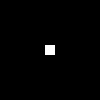
\includegraphics[width=0.5\linewidth]{env_examples/env0.jpg}
    \caption{Example of the simplest environment with a static square.}
    \label{fig:env0}
\end{figure}

I expected the model to overfit very quickly since the state was always identical, and there was a single action that always yielded the best possible reward. The model got to an IoU of 0.94 after around 160,000 time steps, but surprisingly, it started to critically forget shortly after, and it never recovered. Nonetheless, the environment was successfully solved. Since this behavior happened less and less for the more complex environments, I assume the problem was too simple for a complex algorithm such as \texttt{PPO}.

Figure \ref{fig:v0_rew} shows the mean reward per episode during the training. Since an episode always consists of precisely one observation, the highest possible reward is 1 (since that is the highest achievable IoU). The $x$-axis shows the elapsed time steps.

\begin{figure}
    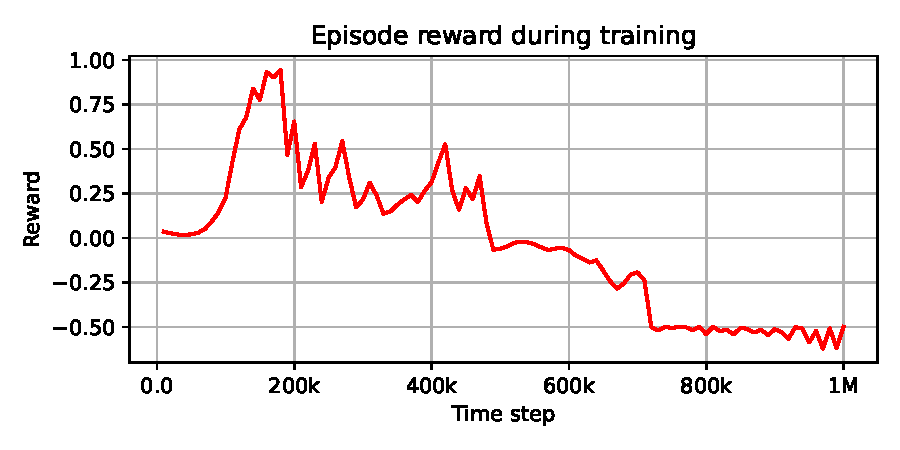
\includegraphics[width=1\linewidth]{graphs/v0.pdf}
    \caption{The mean reward per episode for the simple static square environment. The data was collected by evaluating the agent for 20 episodes after every 10,000 training time steps.}
    \label{fig:v0_rew}
\end{figure}



\section{Randomly placed square of uniform size}
% env v1 %
The next step forward was to make the square move. The initial state was created by placing the square in a randomly chosen position within the image. All the other parameters (reward, action, and algorithm) remain the same. Figure \ref{fig:env1} shows some examples of this environment.

\begin{figure}
    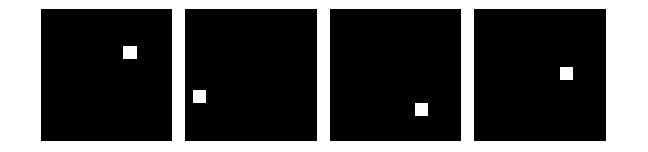
\includegraphics[width=1\linewidth]{env_examples/env1.pdf}
    \caption{Four examples of the environment with a randomly placed square.}
    \label{fig:env1}
\end{figure}

The best model could guess the bounding box's position pretty well, usually within the actual square. However, it struggled with the size even though, again, there was a single correct answer. It even sometimes predicted the width or height of zero, even though that always resulted in a zero reward. Just like the previous model, this one also started to catastrophically forget. Even though the result was not optimal, it showed that the model could handle the movement, so I decided to continue.

\section{Single randomly placed rectangle}
\label{sec:moving_rectangle}
% env v2 %
The following environment was, once again, very similar, the only exception being that the object could now have any size, not just a perfect square of uniform size. Both the placement and size were chosen randomly but with a few constraints. The rectangle could not have a width or height of less than 10 percent of the image, and it could not overflow outside of the image. A few examples are shown in Figure \ref{fig:env2}.

\begin{figure}
    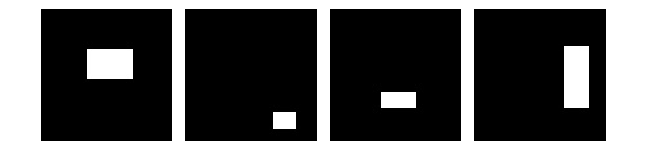
\includegraphics[width=1\linewidth]{env_examples/env2.pdf}
    \caption{Four examples of the environment with a randomly placed rectangle.}
    \label{fig:env2}
\end{figure}

This time, I also wanted to try the other network architecture provided by the SB3 library \texttt{MlpPolicy}, which has a simpler, non-CNN-based architecture (shown in detail in Figure \ref{fig:mlp_policy} in the Appendix). The network has fewer parameters (1.3 million compared to 2.7 million), but for such a simple problem, that could still be more than enough.

The MLP-based policy outperformed the CNN-based one and seemed a lot more stable. While it had some dips in its performance (probably caused by exploration), it always recovered and did not critically forget, as visible in Figure \ref{fig:v2_mlp_cnn}.

\begin{figure}
    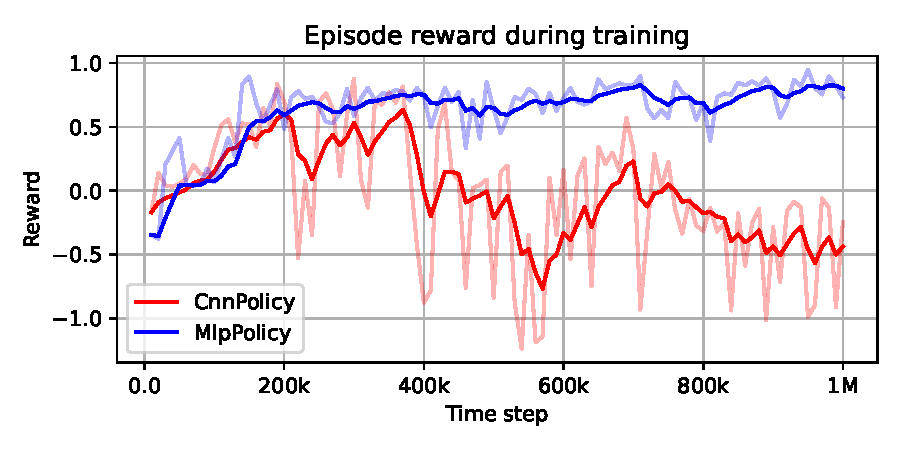
\includegraphics[width=1\linewidth]{graphs/v2_mpl_cnn.pdf}
    \caption{Comparison of the mean reward of the MLP and CNN policies. The data was collected by evaluating the agent for 20 episodes after every 10,000 training time steps. For better clarity, the graph contains both raw values and exponential moving averages.}
    \label{fig:v2_mlp_cnn}
\end{figure}

\section{Multiple rectangles}
\label{sec:multi-rect}
% env v3 %
Since the performance of detecting a single object seemed pretty good, the next logical step was to add more objects. The next environment had the following properties:
\begin{itemize}
    \item State: consists of a binary $100\times100$ pixel image. Five attempts are made at placing a rectangle of a random size in a random place. It is added to the image if it does not overlap with any already placed rectangle. Because of this randomness, the amount of objects changes between episodes; it can be between 1 and 5, but on average, 3.5 objects are present. Four examples can be seen in Figure \ref{fig:env3}.
    \item Action: a tuple of four real numbers representing the bounding box as described in Section \ref{sec:problem_definition}. If the predicted bounding box overlaps with any objects, those objects are erased from the state (in their entirety, even if the prediction does not cover their whole area).
    \item Reward: The reward calculation is similar to the previous environments. If the prediction overlaps an object, its IoU with the guess is the reward (if it overlaps multiple, then the maximum IoU is given). The episode terminates when all objects are removed. The episode is truncated if the number of guesses matches the number of initially placed objects. Note that the model is not directly punished for selecting more than one object. However, since only one reward is given, it is more beneficial to select them separately.
\end{itemize}

\begin{figure}
    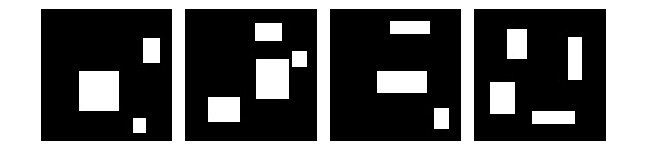
\includegraphics[width=1\linewidth]{env_examples/env3.pdf}
    \caption{Four examples of the environment with multiple randomly placed rectangles}
    \label{fig:env3}
\end{figure}

Again, I tried both MLP and CNN policies. This time, they both performed similarly, stabilizing at a mean reward per episode of around 0.75 after around 400,000 time steps. At first glance, the results might seem just as good as in the previous environment. However, since the episodes lasted multiple time steps (3.5 on average), the maximum possible reward per episode was now around 3.5, whereas before, it was just 1. This poor result was despite both agents doing an average of 3 actions per episode.

\subsection{Different action definition}
\label{subsec:different_rect_repr}

As mentioned in Section \ref{sec:problem_definition}, using four real numbers, there are multiple ways to define a bounding box. Before, I interpreted the action as $(x, y, w, h)$. In this experiment, I changed the meaning to $(x_1, y_1, x_2, y_2)$ or the coordinates of the top-left and bottom-right corners. My thought process was that since convolutions are translation invariant but not scale invariant, it should be easier to find the corners than the entire object whose size is variable.

This change slightly improved the performance of the CNN-based model (from 0.75 to 1) but surprisingly made the MLP-based model worse by around 33 percent.

\subsection{Transfer from previous environment}

Since the previous environment used identical definitions of space and actions, it was possible to reuse its weights in this environment with the potential of transferring some of the learned knowledge. While the transferred agent did start much better, it quickly forgot everything and did not catch up to the agent initialized with random weights.

\subsection{Changing the network architecture}
\label{subsec:arch_change}

The training progressions of the experiments in this section showed a similar trend. They started off learning relatively quickly, making significant progress. After the first 200,000 time steps, the progress slowed down dramatically. This plateauing could hint at the agent being too simple for the environment and unable to learn to interact with it optimally.

Since SB3 uses PyTorch in the background, modifying the underlying neural networks is relatively simple. In the default \texttt{CnnPolicy}, the actor and the critic share a feature extractor with three convolutional layers and one fully connected layer. Then, each of them has a single fully connected layer (for more detail, see Figure \ref{fig:cnn_policy} in the Appendix).

I asked ChatGPT to suggest a slightly larger architecture since designing a neural network architecture is not something I have done previously. It suggested adding an extra fully connected layer to the feature extractor and two fully connected layers to the actor and the critic. This meant that the model now had around 6 million parameters. The new architecture is shown in more detail in the Appendix in Figure \ref{fig:bigger_net_policy}.

This new network was a definite improvement. It outperformed the simple network and continued learning even after more than 7 million episodes. Figure \ref{fig:v3_bigger_net} compares the bigger network and the best \texttt{CnnPolicy} model (the only change between these two trainings was the network architecture).

\begin{figure}
    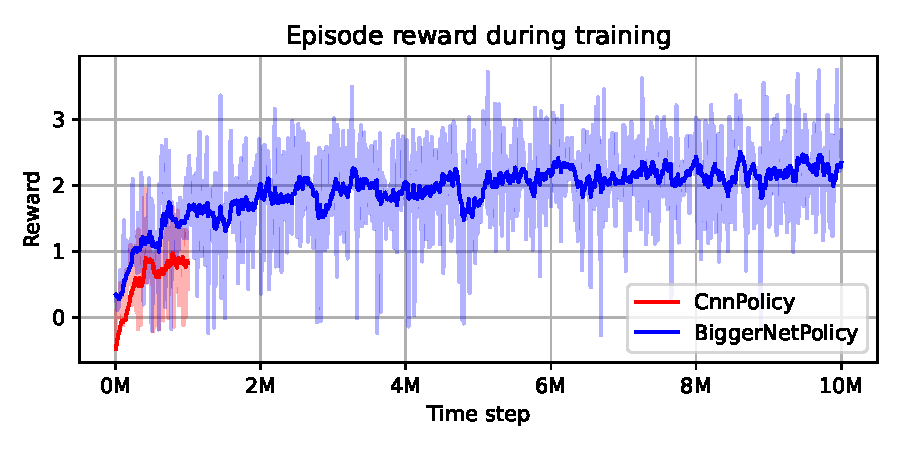
\includegraphics[width=1\linewidth]{graphs/v3_cnn_vs_biggernet.pdf}
    \caption{Comparison of the mean reward of the default \texttt{CnnPolicy} and a bigger network. The data was collected by evaluating the agent for 20 episodes after every 10,000 training time steps. For better clarity, the graph contains both raw values and exponential moving averages.}
    \label{fig:v3_bigger_net}
\end{figure}

The resulting model took around 6 hours to train and reached a mean reward of around 2.1 per episode or an average IoU of 0.6. One problem that brings the average down is that sometimes when the image contained two objects far apart, the model got confused and repeatedly predicted a bounding box between them until the episode was truncated. An example of a situation where this problem occurred can be seen in Figure \ref{fig:v3_stuck}.

\begin{figure}
    \centering
    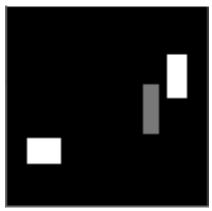
\includegraphics[width=0.5\linewidth]{results/v3_stuck.png}
    \caption{Example of the model getting stuck when two objects are far apart. White rectangles are the actual objects, and grey is the prediction.}
    \label{fig:v3_stuck}
\end{figure}

\section{Different shapes}
\label{sec:different_shaps}
%v4 env%
Now that the model could locate multiple rectangles in a single image with quite a reasonable accuracy, the next step was introducing other shapes. This new environment was identical to the previous one, but there could also be ellipses and triangles instead of just rectangles. Since the rules were still the same, there were an average of 3.5 objects, and their bounding boxes did not collide. Figure \ref{fig:env4} shows some examples of this environment.

\begin{figure}
    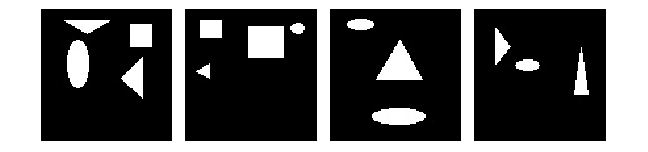
\includegraphics[width=1\linewidth]{env_examples/env4.pdf}
    \caption{Four examples of the environment with multiple different objects}
    \label{fig:env4}
\end{figure}
 
The training on my bigger network started off very similarly to the previous environment, but it never reached quite the same results, stopping at an average reward of around 1.5.

Since the problem was similar to the previous one, I tried using transfer learning with the best model from the previous environment. It started with good results and stayed at a reward of around 2.0 for the rest of the training, only improving slightly.

This result showed me that it was possible to get good results. However, I wanted to avoid transfer learning until the very end because, if needed this early on, it would create a very long and impractical chain of models that depend on one another. For those reasons, I wanted to improve the network further.

\subsection{ResNet-18 feature extractor}
\label{subsec:resnet}

It is common not to create your feature extractor from scratch but instead to use one from an already existing network trained on a similar problem \cite[p. 256]{DLforVisualSystems}.

ResNet is a model architecture first proposed in the paper \textit{Deep Residual Learning for Image Recognition} \cite{ResNet18}. It introduced multiple architecture sizes, such as ResNet-18, ResNet-34, ResNet-50, and more. I decided to try the smallest one since even that would be a significant upgrade over the current feature extractor. The architecture of ResNet-18 can be seen in Figure \ref{fig:resnet}.

\begin{figure}
    \centering
    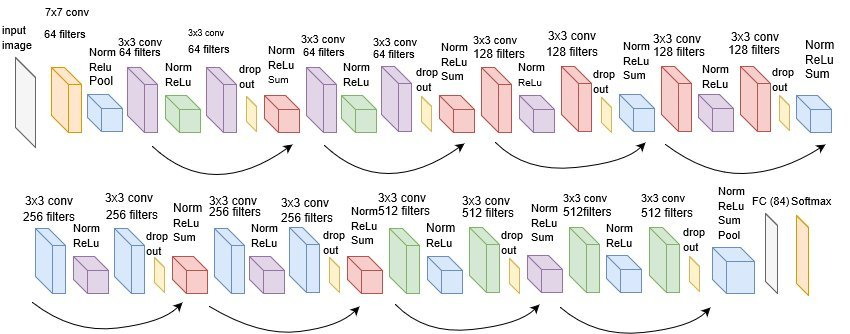
\includegraphics[width=1\linewidth]{diagrams/resnet.png}
    \caption{Architecture of ResNet18. The illustration was taken from \cite{resnet_illustration}. TODO možná si udělám vlastní obrázek, tenhle je hnusnej}
    \label{fig:resnet}
\end{figure}

ResNet-18 is a convolutional neural network with 18 layers and residual (skip) connections that help mitigate vanishing gradients. Each convolution is typically followed by batch normalization. While the original ResNet ends with an average pooling layer, the PyTorch implementation uses an adaptive average pooling layer, which ensures a fixed-size output regardless of the input dimensions.

A slight complication is that ResNet-18 takes colored images (3 channels) as input, while the environment uses binary images (1 channel). To solve this issue, I added a convolutional layer at the beginning with a kernel of size $1\times1\times3$, which creates three feature maps from the one-channel image. The entire architecture is shown in the Appendix in Figure \ref{fig:resnet_arch}.

It is also important to note that the ResNet-18 weights provided by PyTorch were pre-trained on the ImageNet-1k v1 dataset \cite{torchvision2016}. This dataset differs from our use case, which could mean the knowledge will not transfer well.

I tried again in the same environment. At first, I used the weights from PyTorch and froze them because I thought this would speed up the training. The results were very poor. Next, I ran the same test, but this time, the weights were no longer frozen and could thus adapt to the new problem. This time, the training went much better, reaching a reward of around 2.8 in less than 2.5 million time steps. Lastly, I also wanted to test whether the pre-trained weights made any difference compared to randomly initialized weights. The comparison of these three experiments and the best result reached with the previous architecture can be seen in Figure \ref{fig:v4_resnet_graph}. 

\begin{figure}
    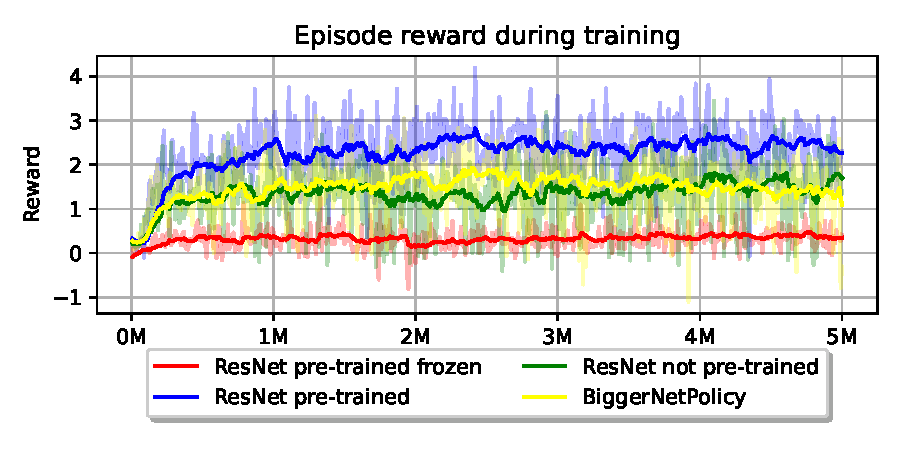
\includegraphics[width=1\linewidth]{graphs/v4_resnet_graph.pdf}
    \caption{Comparison of the mean reward of the pre-trained frozen, pre-trained fine-tunable, and not pre-trained ResNet-18 based agents with the previous architecture. The data was collected by evaluating the agent for 20 episodes after every 10,000 training time steps. For better clarity, the graph contains both raw values and exponential moving averages.}
    \label{fig:v4_resnet_graph}
\end{figure}

While the performance improvement was significant, it slowed down the training notably. It took around 2.5 hours for one million time steps, which was around three times slower than before.

\section{Hollow shapes}
%env 5%
One considerable simplification we are currently undertaking is that each position in the image can belong to at most one object. To put one object inside another, we need to mark only its edge; otherwise, the inside object would not be visible. The only change in this environment is that the objects are drawn as outlines, as visible in Figure \ref{fig:env5}.

\begin{figure}
    \centering
    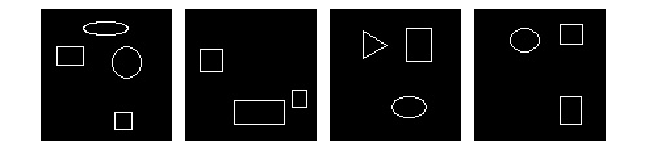
\includegraphics[width=1\linewidth]{env_examples/env5.pdf}
    \caption{Four examples of the environment with multiple shapes of objects}
    \label{fig:env5}
\end{figure}
 
This change had little to no effect on the training progression.

\section{Bigger images}
%env 6%
At this point, I was working with images of size $100\times100$ pixels, whereas AIVA currently uses a resolution of $1920\times1080$ pixels. Since we only need to locate the objects, which should not require pixel-sized details, some downscaling is possible, but squashing the image down to $100\times100$ pixels would likely be too much. Because of this, I wanted to experiment with larger image states.

Thanks to the aforementioned adaptive average pooling layer used in the ResNet-18 feature extractor, changing the image size would not require manual network architecture modifications.

Due to hardware limitations (GPU memory), the largest state with which I could get a training running was $640\times480$ pixels. However, even then, the training speed slowdown was so significant that I decided to continue with a state size of $200\times200$ pixels (this slowed down the training around two times).

The size increase did not cause significant differences in the training progression. However, since the image was bigger than before, more objects were placed (7 on average). Unfortunately, this caused the reward per object to drop significantly. The model learned to place large bounding box predictions in relevant areas. This strategy resulted in a positive reward but was far from optimal since it usually removed multiple objects simultaneously. The likely cause was that the current reward function did not punish selecting multiple objects at once directly. I came up with two new algorithms to calculate the reward in the case where the guess bounding box intersected multiple objects:

\begin{itemize}
    \item Find all objects that intersect with the guess. Find the object with the biggest overlap and calculate its IoU. Calculate the sum of the overlap areas of all the other intersecting objects with the guess, divide this sum by the guess' areas, and subtract it from the IoU.
    \item Calculate IoUs of all the objects that intersect with the guess. The reward is the biggest IoU minus the sum of all the other IoUs multiplied by a constant (I chose ten).
\end{itemize}

The first option did help, bringing the per-object IoU from 0.5 to around 0.6. The second one had a very minimal impact. While IoU of 0.6 is usually considered acceptable \cite[p. 291]{DLforVisualSystems}, this experiment showed me that my current solution had problems even with an object count of less than 10, which is not acceptable since an average website probably contains closer to 100 objects.

\section{Hierarchical environment}
\label{sec:hierarchical-env}

So far, all the environments have had objects that did not intersect. They were independent; thus, the order in which they were selected did not matter. This, of course, differs from how actual websites look. They have a hierarchy of objects (one can contain many others). The next step was to create an environment that would represent this more faithfully.

At first, I tried to use the same technique as before -- randomly attempting to place objects that do not overlap, but this time, I allowed such overlaps where one object was entirely inside another. This strategy did not work well; the number of objects differed significantly between attempts, they were often placed very close to one another, and the depth of the hierarchy was shallow. So, instead, I created a generator that directly created a tree-like structure.

The generator starts with a root object that encloses the whole image, then it selects an area inside with a random offset to the parent object and randomly selects the number of children, their sizes, and the spacing between them. The algorithm then does this recursively for each child. It is also possible to customize the maximum depth, the minimum size of an object, minimum spacing, and children count. Some examples of this new generation are shown in Figure \ref{fig:env7}

\begin{figure}
    \centering
    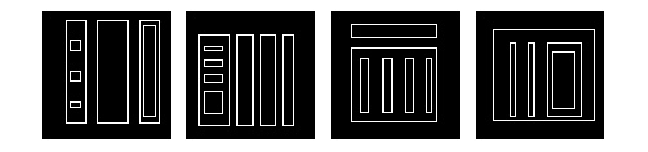
\includegraphics[width=1\linewidth]{env_examples/env7.pdf}
    \caption{Four examples of the new hierarchical environment}
    \label{fig:env7}
\end{figure}

A new reward function was needed as well. I came up with the following method. First, find all objects the guess intersects with or fully encloses; if none exist, include objects that fully enclose the guess (there will always be at least the root). If there is just one such object, the reward is the IoU of this object with the guess minus the percentage of its area occupied by its children that have not been guessed yet (this is to discourage selecting objects that still have children). This object is then removed (including all of its children). If multiple intersecting objects exist, the one deepest in the hierarchy is chosen, and the same calculation is performed. The episode ends when the root object is removed.

I tested this new environment by training two new models. One from scratch and the other transferred from the previous environment. After around 7 million time steps, they both managed to get an average reward of about 2. The transferred model performed slightly better, but not by much. From the testing, it was clear that the model learned that placing long bounding boxes of zero width would almost always result in a nonnegative reward. The model did not explore enough to realize it could do much better.

\subsection{Manual hyperparameter tuning}

One thing I have not yet experimented with was hyperparameter tuning. This was a perfect opportunity since I needed to encourage the model to explore more. I manually tried changing each of the following parameters:

\begin{itemize}
    \item The discount factor $\gamma$ (described in Section \ref{sec:goal}) -- By default, this parameter is set to 0.99, but in our case, discounting does not make sense. Because of how the environment works, the maximum number of steps for the episode is capped, and an ideal policy will use up all of them. Thus, discounting is unnecessary, and $\gamma$ should be set to 1.
    \item Entropy loss coefficient $c_2$ -- The PPO loss function contains an entropy bonus that rewards less deterministic policies. Increasing it should thus lead to a more stochastic model and more exploration~\cite{PPO_paper}. By default, this hyperparameter is set to 0.
    \item Clipping range $\epsilon$ -- One of the main benefits of PPO is its clipping function that prevents large updates to the policy and value function, which should prevent it from \enquote{jumping off a cliff}~\cite{PPO_paper}. By increasing it, the training might become more unstable, but it also might help to get out of local maxima.
    \item Learning rate $\varepsilon$ -- When updating the policy network, the gradient is multiplied by the learning rate. A higher learning rate should make the training faster, but at the same time, the jumps are more significant, which can lead to unstable learning.
\end{itemize}

I tried both lowering and increasing each of these parameters, but unfortunately, none of the changes had a more significant positive impact. Lowering $\gamma$ and increasing the clip range led to slightly better results, but only a little. Looking back at these attempts, I believe the problem was that I did not understand how the parameters should be changed, so I chose some values that looked good without any more sophisticated strategy.

Later, when I discovered Optuna (see Section \ref{sec:optuna}), I also attempted an automated hyperparameter search, but even that did not lead to much progress. Since I did not have many ideas for improving the training further, I decided to try a completely different approach.

\section{Switching to discrete actions}
\label{sec:iterative}

Since the results of the previous approach, which guessed bounding boxes directly (one action = one prediction), did not work well, especially in a more complex environment, I wanted to try a different approach. In \cite{rl_object_detection}, Samiei and Li describe and compare two previously proposed approaches for object detection using reinforcement learning, both using a discrete action space. Both of these methods start with a bounding box spanning the entire image. Then, the agent chooses actions that modify this selection repeatedly. Once the model is satisfied with the prediction,  it selects the \texttt{trigger} action, confirming the selection (and ending the episode in case of a single object detection). The initial state is the entire searched image (scaled to some fixed size). After each action, the state is modified only to include the current selection.

The first method, initially described in~\cite{hierarchical_od_with_drl}, has five movement actions (each resulting in zooming towards one of the corners or the center of the image) and the trigger action. It showed promising results on a single object, single-class object detection. However, it cannot be used since it only produces bounding boxes with the same aspect ratio as the image.

The second method, initially described in~\cite{iterative_od_with_rl}, uses a similar approach. However, instead of five actions for zooming in different areas, it has a total of eight movement actions (plus the trigger), four of which move the bounding box (up, down, left, and right), two change the size (zoom in, zoom out) and two change the aspect-ratio (making the selection fatter or taller). These actions allow for way more flexibility, although some bounding boxes are still impossible because the changes are not continuous. However, if the size change is small enough, it should be fine, as we do not need pixel-perfect predictions. Figure \ref{fig:exmaple_from_paper} shows an example of one episode using this approach.

\begin{figure}
    \centering
    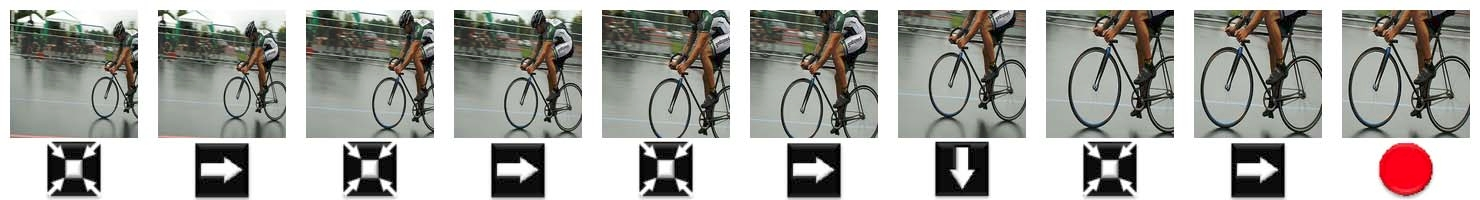
\includegraphics[width=1\linewidth]{diagrams/45.jpg}
    \caption{Example of taken actions to locate an object~\cite{iterative_od_with_rl}}
    \label{fig:exmaple_from_paper}
\end{figure}

As mentioned prior, the observation space is once again an image. The original paper~\cite{iterative_od_with_rl} also used a vector of ten previous one-hot encoded actions, but~\cite{rl_object_detection} found that including them did not change the outcome.

I implemented a simpler version of this approach with only four actions, each shrinking the bounding box by some fixed percentage from one of the four sides. This change simplifies the problem while keeping the ability to create predictions of any size.

The suggested reward function compares the IoU of the selection before and after an action is taken and gives a reward of +1 if the action improved the guess and -1 if not. When the trigger action is selected, a reward of $\eta$ is given if the resulting IoU is over some threshold $\tau$, $-\eta$ otherwise. The suggested values are $\eta=3$, $\tau=0.5$.

This reward function is suitable for single object detection. Unfortunately, when more than one object is present, it is difficult to determine whether the action improved the selection since it can differ for each object. For this reason, I started my experiment with a simpler semi-sparse reward function, which only rewards the trigger actions. The same calculation was used as in the continuous-action environment equivalents.

\section{Single randomly placed rectangle with discrete actions}

To test this new approach, I modified the environment described in Section \ref{sec:moving_rectangle}, which contains just a single rectangle. The model learned to find the rectangle quickly, but the accuracy was not great, mainly because the selection shrinking was too large (one step shrunk the bounding box by 15 percent). The accuracy improved when I lowered it to just 5 percent, but it took way too many steps per episode (around 60), which could slow down the inference.

Compared to the previous approach in the same environment, the training did take around ten times as many time steps to get to the same reward, but this is to be expected since suddenly a single guess required 30 to 50 time steps instead of just one.

\section{Multiple rectangles with discrete actions}

Since the results in the simple single-rectangle environment were satisfactory, I continued and modified the environment described in Section \ref{sec:multi-rect} to use discrete actions. To account for the problematic accuracy caused by large steps shown in the previous environment, I implemented two actions per direction, one shrinking the bounding box by 15 percent and one by just 2.5 percent. This change does make the task slightly more complex, but at the same time, allows for precise predictions with a lower number of steps.

This is the environment where, with the previous approach, I had to switch to the bigger network. This time, I went directly with the ResNet-18-based network. This combination worked well, reaching the same reward of 2.1 in only around 700,000 time steps compared to the 10,000,000 with the previous approach, even though one episode took around 80 time steps compared to 3.5.

\section{Hierarchical environment with discrete actions}

Seeing the success of the new approach, I decided to skip to the hierarchical environment described in Section \ref{sec:hierarchical-env}, which I could not solve using continuous actions.

\subsection{Changing to dense reward function}

Unfortunately, the new approach did not help. The agent struggled even to reach positive rewards. I decided to try and get my reward function closer to the one described in~\cite{iterative_od_with_rl}. The main change was going from a semi-sparse function (only giving rewards for trigger actions) to a dense function (rewarding every action).

I came up with the following. After each interaction, find all leaf elements (with no children) that overlap with the current selection. If there are none, reward zero. Otherwise, find the element that has the highest IoU with the current selection. If the selected action is the trigger action and the IoU is over 0.5, reward 3, else -3. In both cases, remove the element. If it is not the trigger action, compare the IoU with the IoU after the previous action and reward the difference. The episode ends once all nodes are removed.

After some experimenting, I changed the reward function for the trigger action not to give a fixed constant value but instead to award 3 times the selection IoU, since otherwise there would be no incentive to exceed the threshold IoU of 0.5.

\subsection{Automated hyperparameter tuning}

Since I was not seeing much progress, I decided to revisit hyperparameter tuning, but this time using Optuna (see Section \ref{sec:optuna}).

I ran a study of 200 trials, each running 200,000 time steps (if not pruned). The tuning took around 24 hours, although the final best hyperparameters were found in trial 23 after only 3 hours. According to this study, the most important hyperparameter was the learning rate. Optuna found that using about a tenth of the default learning rate with linear decay made quite a significant difference.

The new reward function and hyperparameters brought the average episode reward from barely over zero to over twelve in less than one million training time steps. Since the current environment generated, on average, 3.9 objects, and the maximum reward per object was 4 (1 for shrinking actions, 3 for the trigger actions), this result meant an average IoU of over 0.75.

After increasing the average amount of objects per image to 6.3 and another two days of hyperparameter tuning, the reward got to over 20 or an IoU of almost 0.8 per object. This result showed me that the approach with discrete actions scaled well even with more objects.

Interestingly, one of the tunable parameters was the size of the actor and critic networks. In both of the tunings, this parameter was deemed as very unimportant. In that later one, the best result was achieved using the smallest architecture of only one layer of 64 neurons. Because of this result, I reverted to the simple \texttt{CnnPolicy} provided by SB3.

\section{Rectangles based on a website screenshot}
%v8 env%

Now that I could train a model that correctly finds elements in a hierarchical environment, the next step was to move to more realistic data. Instead of generating rectangles in random places, I wanted them to reflect real websites.

\subsection{Dataset}
\label{subsec:dataset}

Ideally, I would like to find a dataset containing screenshots of websites and annotations of elements on that screenshot. Such datasets exist, for example, \cite{roboflow-dataset-1} and \cite{roboflow-dataset-2}. Unfortunately, they are usually small (at most a bit over 1,000 images), contain just the \enquote{leaf} elements (not bigger sections such as spans or divs), and often contain straight-up wrong or duplicate annotations. After all, this thesis aims to train a DL-based model that does not need such a dataset precisely for these reasons.

Instead, I chose to use a dataset that contains just the screenshots and then somehow find the approximate locations of the elements using a CV-based function. The best public dataset I found was~\cite{aydos2020}. This dataset contains 20,000 website screenshots split into four categories: machinery, music, sport, and tourism (the original purpose of the dataset is to classify these categories). It offers the screenshots in two sizes, $224\times224$ pixels (too small for our use case) and $1440\times900$ pixels.

For each image, I then find the elements using the following method. First, convert the image to grayscale and apply a bilateral filter (which helps to eliminate textured backgrounds that would mess up edge detection). Next, locate edges using the Canny edge detection algorithm, and connect close ones using morphological closing. Lastly, find connected components and filter out those that are too small. Then, create a new black image the same size as the original screenshot and add white rectangles corresponding to the found objects. The result is similar to what we generated in the last environment, but based on an actual website. Since the original image is not given to the model, it is not a problem if we fail to detect some objects. The individual steps are shown in Figure \ref{fig:simple-detector}.

\begin{figure}
    \centering
    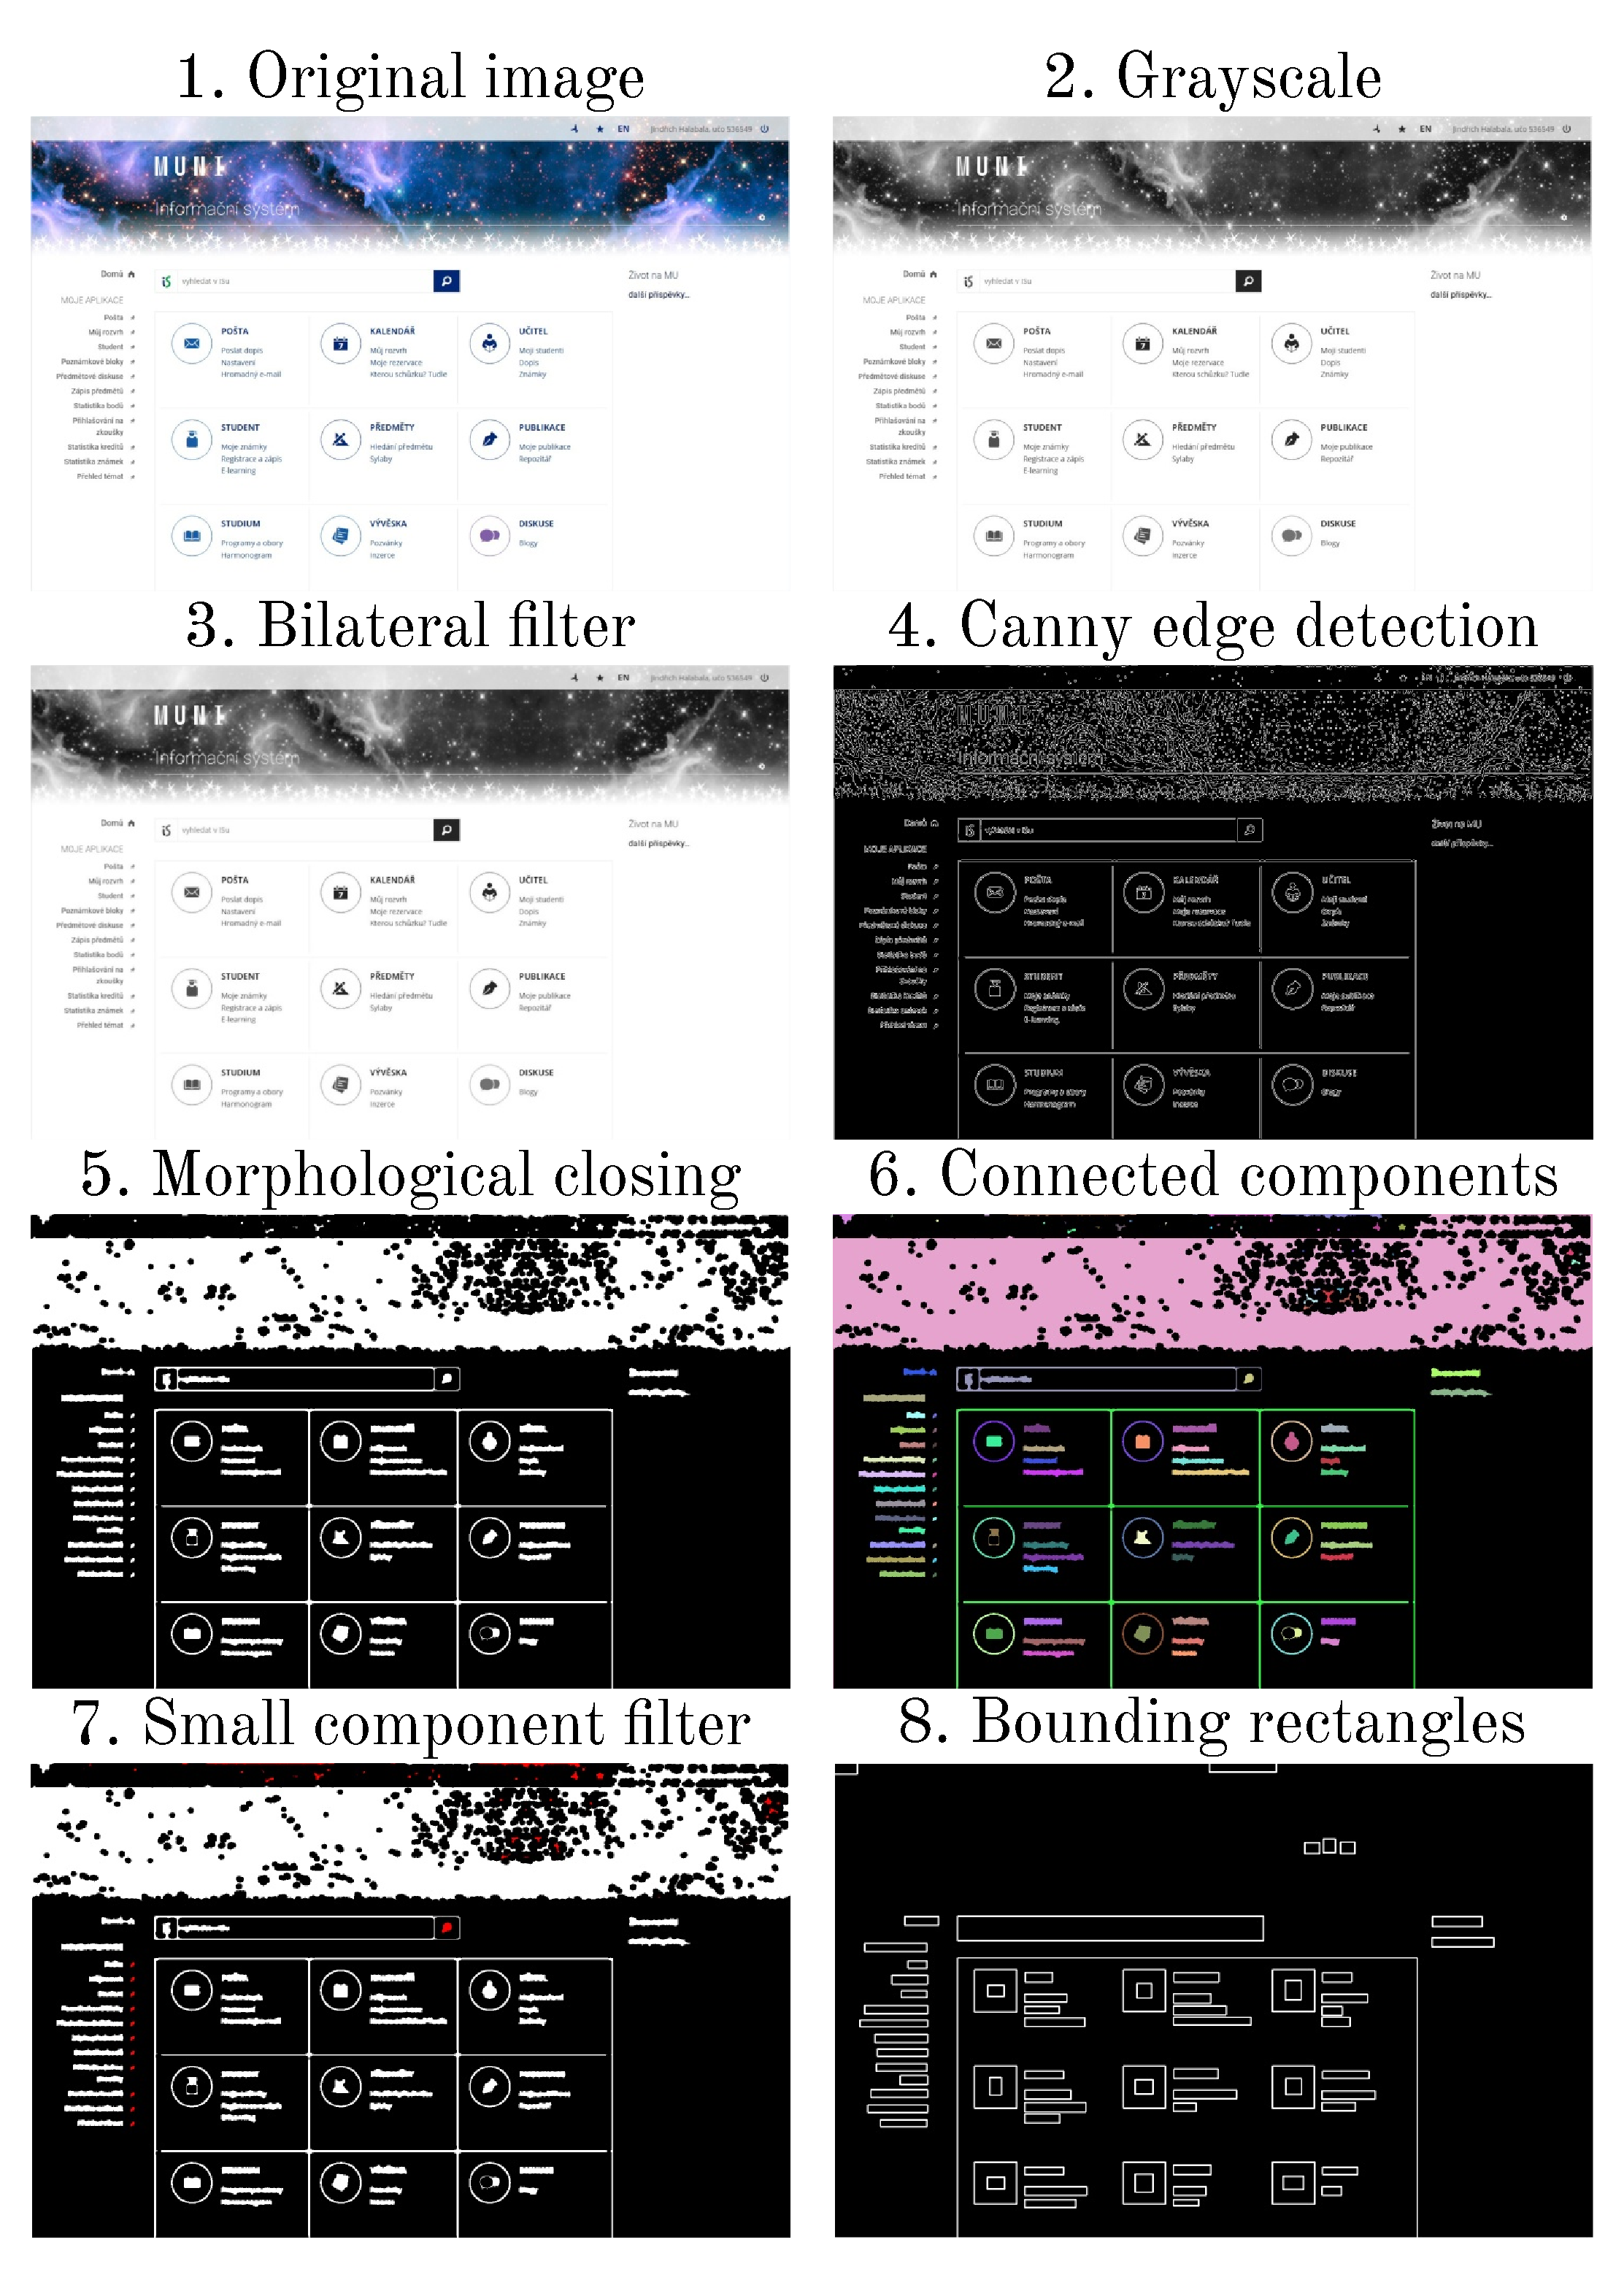
\includegraphics[width=1\linewidth]{diagrams/simple_detector.pdf}
    \caption{The steps taken when creating a state from an image.}
    \label{fig:simple-detector}
\end{figure}

I could locate an average of 26 objects per image using this method. If we aim for an IoU of 0.7 with the current reward function, the goal for this environment should be a reward of around 72 per episode. A few examples of the initial states are shown in Figure \ref{fig:env8}.

\begin{figure}
    \centering
    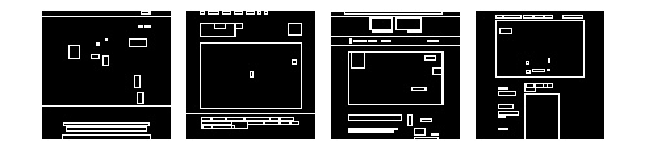
\includegraphics[width=1\linewidth]{env_examples/env8.pdf}
    \caption{Four examples of the environment where rectangles are based on real websites.}
    \label{fig:env8}
\end{figure}

\subsection{Reward function}

At first, I reused the same reward function as in the last environment. There, with less than 10 objects, it worked reasonably well. However, with over 20, the agent was again unable to understand the environment. The resulting model repeatedly placed large predictions until the episode ended.

To combat this, I changed the logic to involve not only leaf objects. If the first prediction was large and had the best IoU with the root element, the episode would end instantly. Unfortunately, this brought yet another problem. Since the initial selection is identical to the root element, the next couple of actions would always result in negative rewards. The selection would worsen until it became small enough to have better IoU with another element. This might confuse the agent, so I added another condition that removed the root element from these calculations unless it was the last remaining one.

After this change, I reached an average reward of around 20 per episode.

\subsection{Curriculum learning}

Curriculum learning is a technique where the agent is trained on data of increasing difficulty. Since I was still the one creating the states, this would be relatively easy to do. I would only add the $n$ biggest bounding boxes when making the image. At the start, I set $n=3$. I then started saving the given rewards into an array, and once 100 of them were collected, I would calculate the average, and if it were over some threshold (I started with 0.7), I would increase $n$ by one.

After running this environment for 20,000,000 time steps, the agent beat the previous training by about 5. However, more importantly, the reward did not plateau and kept increasing even after such long training.

Later on, I found some more errors in the environment. Namely, since the reward for non-trigger actions was calculated as a difference between the current best IoU and the last best IoU, it did not work well on the first action after a trigger action.
Another interesting issue was image scaling. Since the RL algorithms require the same-sized input every time, it was necessary to scale the selection to the state size. The problem is that based on the interpolation method used when scaling, some thin lines could disappear, making them invisible to the agent. Especially problematic was that this scaling could be both up-scaling and down-scaling or even both, one for each axis. Ultimately, I solved this by scaling separately for each axis and choosing a different interpolation method based on the situation.

After fixing these issues, the agent reached an average reward of 55 per episode.

\subsection{Tolerant Intersection over Union}
\label{subsec:eval_metric}

Until this point, I was using the IoU metric to evaluate the goodness of a selection. It is the standard for bounding box prediction evaluation compared to the ground truth. It works well in classic object detection tasks where most objects are of a similar size. However, that is not the case in this problem. Some objects can take up most of the image, while others can take up less than 0.01 percent of the screen area.

IoU calculates relative errors. This behavior does not reflect my end goal. I care more about absolute differences than relative ones. An error of 2 pixels on a small element is usually not a problem, even though it is a lot relative to its size. An error of 50 pixels is a problem even for a large element, even though it is not much relative to its size. For this reason, I wanted to experiment with other metrics that could better reflect my requirements.

Since the agent currently only receives the zoomed-in view of the image, using a metric that is not purely relative would break the Markov property. The model cannot know if it is zoomed in a lot on a small object or zoomed in a little on a large object. To fix this problem, I expanded the observation space also to include the coordinates of the current view window. This meant changing the observation space to the \texttt{Dict} Gymnasium type and creating a new feature extractor. The entire architecture of this new network is shown in Figure \ref{fig:multiinput_arch} in the Appendix.

This change sped up the training significantly, reaching a stable evaluation score of 60 in less than a third of the time steps and eventually reaching a score of over 70. This difference was somewhat surprising to me since, with IoU, this information should not be necessary.

The first metric I came up with is Tolerant Intersection over Union. It has an extra tolerance parameter. Before the IoU calculation, the edges of the two bounding boxes are moved closer together by, at most, this (absolute, not relative) tolerance value. The result is a weighted sum of the IoU of the original bounding boxes and the modified ones to still slightly prefer a perfect match.

This new metric solved the issue of small bounding boxes being very sensitive, reducing the average episode length by almost a hundred time steps to around 750. On the other hand, it did not improve the bad selections of large bounding boxes, which makes sense because the metric can never produce a worse score than regular IoU.

\subsection{Absolute Sigmoid Score metric}

Since the Tolerant IoU metric still performed poorly on large bounding boxes, I wanted to construct a metric that would rely solely on the absolute differences between the bounding boxes and not consider their size.

The Absolute Sigmoid Score metric computes the differences between the minimum $x$ and $y$ coordinates of the two boxes, the maximum $x$ and $y$ coordinates, and the $x$ and $y$ coordinates of their centers. The sum of these differences (marked as $\text{Diff}( b_1, b_2)$ in the formula below) is then passed through a descending sigmoid function. The sigmoid binds the result to the $[0,1]$ interval and captures the intuition that minor differences should be penalized less. The sigmoid function has two parameters, $\alpha$, which controls the steepness of the sigmoid, and $\theta$, which shifts the sigmoid (I used values $\alpha = 2.8$ and $\theta = 0.5$). To ensure that a perfect match always yields a score of one (regardless of $\alpha$ and $\theta$), the result is divided by the value of the sigmoid at a difference of zero.

\begin{equation}
\begin{split}
    \sigma(x) & = \frac{1}{1+e^{-x}} \\
    \text{AbsSigScore}( b_1, b_2) & = \frac{1-\sigma(\alpha\cdot(\text{Diff}( b_1, b_2)-\theta))}{1-\sigma(-\alpha\cdot\theta)}
\end{split}
\end{equation}

I struggled to find a suitable threshold of where to consider the score good enough to increase the difficulty of the curriculum learning. 0.85 was way too low, and the model's predictions were bad; 0.9 was too high, and the model did not progress. It is possible that with different parameters of $\alpha$ and $\theta$, this metric could be suitable. Nevertheless, for the rest of the experiments, I returned to TIoU.

\subsection{Selection padding}

One potential issue I noticed when debugging the environment was that the agent sees only the current selection. Since the objects are only represented by their outline, the agent can no longer see one of the object's edges if it overshoots while shrinking the selection. Since the agent is memoryless, this could be an issue. I solved this by expanding the observation by a fixed percentage on each side to include some extra area around the selection.

While the final result after 20 million training time steps was almost identical (stable evaluation score of around 80 per episode), it did learn faster, especially at the beginning.

\section{Finding objects in a real image}
%v9 env%

The previous environment has shown that it is possible to train a model that can find objects even in relatively complex hierarchies. However, it was still locating only rectangles in a heavily preprocessed image. This preprocessing required finding all the objects first using a different method, making the actual model somewhat pointless. The next step was creating an environment with only a simple image preprocessing that does not require knowing the locations of all the objects. It takes an image of a website, locates edges, and inflates them using morphological dilation. Figure \ref{fig:env9} shows some examples of the state the model receives.

Besides changing the observation, this environment was similar to the previous one. The reward was still calculated based on ground truth labels, but this time, I used a more advanced CV-based detector (described in Section \ref{sec:trad_cv_detector}) to make the reward function more accurate. This raised the average count of objects per image to 32.4, meaning that the maximum average reward per episode was 129.6, and the goal was to reach 90 per episode (TIoU of 0.7).

\begin{figure}
    \centering
    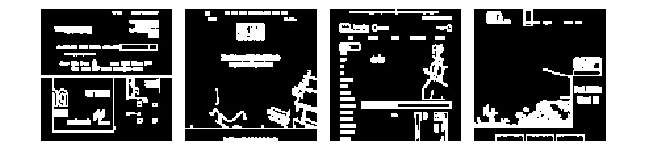
\includegraphics[width=1\linewidth]{env_examples/env9.pdf}
    \caption{Four examples of the environment where the state is a slightly preprocessed image.}
    \label{fig:env9}
\end{figure}

When running a training in this environment, using the same set-up that solved the previous environment, the resulting agent reached a top score of around 46.

The first change I made was to how the scaling of the image was done. In the previous environments, the image was always binary. This was because the objects were marked by only a one-pixel outline, which would often nearly disappear when a significant downscaling was applied. Here, this was no longer the case. By allowing the use of all 256 possible pixel values, the model could get some extra information and allow it to see finer detail. This change brought the average episode reward from 46 to 53.

\subsection{Changing the feature extractor}

Back in Section \ref{sec:different_shaps}, we saw that changing the shapes of the located objects required a larger feature extractor. As a reminder, since changing the action space to being discrete, all the environments were solved using a network with a very simple, not pretrained feature extractor with only three convolutional layers. Since the score dropped significantly when more complex objects were introduced, a bigger extractor could help.

When using the bigger network developed in Subsection \ref{subsec:arch_change} (modified to also take the selection's coordinates), the score increased from 53 to 62. Surprisingly, when trying the ResNet-based architecture (Subsection \ref{subsec:resnet}) the model quickly dropped to a score of zero and never recovered. TODO: try this training again because it is sus.



\chapter{Comparison with other methods}

In the previous chapter, I described the development of a GUI element detector trained using deep reinforcement learning. While this demonstrated that the RL-based approach is feasible, it did not assess whether it offers advantages over traditional methods. In this chapter, I present two prototype detectors based on conventional techniques and compare all three solutions across multiple criteria.

\section{Traditional CV-based detector}
\label{sec:trad_cv_detector}

To create a detector based purely on traditional computer vision algorithms with no ML, I mainly combined techniques described in Section \ref{sec:traditionalCV} to improve my detector described in Subsection \ref{subsec:dataset}. It uses Canny edge detection followed by Suzuki-Abe contour tracking to find potential objects. These are then filtered based on multiple criteria to hopefully only end with actual objects. The entire algorithm is described in detail in the Appendix in Chapter \ref{ap:cv}. The implementation uses the OpenCV library\footnote{\url{https://opencv.org/}} for the image processing.

The two most problematic element types I encountered in the implementation were text and raster images. Unlike other elements, text is not a single large area of pixels but instead many small elements for each letter. It can be challenging to distinguish between a letter contour and one of random noise. To minimize this issue, I used morphological dilation and merged close letters. While this helps, it also creates inconsistencies where large letters are an element each, while smaller ones are merged into a single element.

Raster images are problematic because they contain many edges of irregular sizes, which are unimportant for the element detection. This is especially hard to eliminate when the website uses an image as a background and its edges interfere with the edges of actual elements.

\section{Supervised DL-based detector}

The second common approach for object detection, especially for more complex images, is using deep convolutional neural networks capable of predicting a variable number of bounding boxes trained using supervised learning.

I chose not to implement such a model from scratch, since that alone would likely be enough for a thesis. Instead, I have opted for YOLOv8 \cite{yolov8_ultralytics}. It was developed by Ultralytics\footnote{\url{https://www.ultralytics.com/}} in 2023. YOLOv8 is a collection of pre-trained models for various tasks and of multiple sizes (ranging from 2.7 to 99.1 million parameters) \cite{ultralytics-docs}. Specifically, I used the smallest object detection model \texttt{YOLOv8n}. Newer versions have been released since, but I do have some past experience with YOLOv8, and it has been confirmed to work with GUI elements \cite{GUI_YOLO_comparison}. 

The model is pretrained on the COCO dataset \cite{COCO} and must be fine-tuned for the specific purpose. As mentioned previously, datasets for my task are limited, so for this prototype, I decided to create my own dataset. To do so, I used my CV-based detector (see Section \ref{sec:trad_cv_detector}) and labeled 10,000 images from the WebScreenshots dataset \cite{aydos2020}. Please note that this makes any accuracy comparisons between these two detectors completely invalid, since the YOLOv8 model is essentially learning to copy my current detector and can not thus produce better results. However, since all three compared detectors are prototypes, this should not matter. We can assume that if the model learns well with this mocked dataset, it would also learn similarly well with a real one.

Fine-tuning the model is extremely simple. Using the Python Ultralytics API, an instance of the \texttt{YOLO} class is created with the path to a pretrained model. Next, the \texttt{train} method is called with the path to the dataset. Specifying the epoch count, early stopping criteria, initial learning rate, and some other hyperparameters is possible. However, the library calculates suitable values if not provided. Ultralytics also provides a command-line interface.

\section{Challenges of comparing the detectors}

Before comparing the three detectors, it is important to note that each is at a very different level of maturity. The RL and CV-based detectors were created by me with varying amounts of knowledge of each topic and varying amounts of time. The DL-based detector was created by professionals and only fine-tuned by me.

These prototypes should be sufficient to compare the used concepts and draw attention to their main benefits and problems. However, if one were to look for a specific detector to use in an application such as AIVA, more detailed comparisons should be done with specific existing detectors.

\section{Accuracy}

In classical object detection tasks, accuracy is measured by comparing the predictions with some ground truth labels. However, in the case of UI element detection, this can be somewhat problematic as multiple correct answers might exist. For example, a paragraph of text can be detected as a single element, as one element for each row, one for each word, or even one for each letter. We may prefer one of these options over the others, but none of them is inherently wrong. For this reason and the reasons described in the previous section, I won't be including any numerical data in this section.

TODO: See some predictions and try to spot common mistakes for each detector.

\section{Speed}

For real-time applications, the speed of a detector is crucial. During a single test, AIVA might localize the elements more than a hundred times, meaning it has a high effect on how long a test execution takes.

The prediction times on the YOLO-based detector were by far the fastest. The median prediction time was 12 ms on the GPU and 30 ms on the CPU. The time did depend on the number of objects detected, though the differences were small (11 ms for 20 objects, 15 ms for 80 objects). The very first prediction is a lot slower, taking around 1.5 s.

The CV-based detector was slower, with a median prediction time of 144 ms. Here, the object count played a bigger role (125 ms for 20 objects, 200 ms for 80 objects). On the other hand, the detector does not require any initialization, making the time to first prediction faster than that of the YOLO-based detector. If speed were the primary goal, it could definitely be optimized further. For example, the bilateral filter takes up over 46 percent of the runtime. Another 17 percent is used on thousands of operations with bounding boxes, many of which could likely be removed or calculated in a faster way.

The RL-based detector is slow. While each step of the model only takes a bit over 1 ms on the GPU (around 2 ms on the CPU), this approach also requires simulating the environment (around 0.5 ms per step) and, most crucially, every bounding box prediction requires anywhere from 20 to 40 steps. That means over 100 ms per bounding box and multiple seconds for the whole image.

I believe there are ways to bring this time down. Modifying the shrink amounts or adding even more actions for different levels of shrinking could significantly reduce the step count. With the continuous actions attempted at the beginning, only a single step per object would be required. A combination of discrete and continuous actions, where the model would pick a direction and amount of shrinkage, could also work. Unfortunately, the SB3 library currently does not support mixed action spaces.

\section{Data requirements}

Try training the RL-based detector and YOLO detector on datasets to sizes 100, 1,000, and 10,000 (current) and see the difference.


\section{Implementation difficulty}

The final criterion I want to assess is the difficulty of implementing a detector using each approach. While this is very subjective, I believe it to be one of the most important for actual usage.

Reinforcement learning is not usually used for element detection. Because of this, I had to implement most of the parts (environments, reward functions, networks) myself. There is also very little information available on reinforcement learning with image input. While some famous image-based environments exist (namely, Atari games and the OpenAI robot fetch), most RL environments, tutorials, and projects use much lower-dimensional observations. This meant a lot of experimenting, often with mixed results.

However, supervised learning-based object detection is a very well-explored subject. Many datasets and ready-to-use models exist, along with tutorials on how to use them, and new papers and versions of these models are released regularly. Once I created the dataset, it took me under 3 hours, including training, to get the first decent YOLOv8 prototype. Of course, if one were to implement their model from scratch, it would take much longer, but I still believe it would be more straightforward than when using RL.

With CV-based detectors, it is more complicated. From my experience, I can confirm that a person with basic image processing knowledge can create a CV-based detector that works well on simple GUIs within hours. But then again, making it work on more complex GUIs can take hours of tedious finding of ideal thresholds and parameters, only to find another case where the current setup fails. The most significant advantage here is that the whole algorithm is very transparent and debuggable, which makes fixing problems much more straightforward than with black-box machine learning.

I believe that the most time-efficient way to implement an element detector would be to use existing ML-based models for detecting difficult-to-process elements (namely, an OCR for texts and a YOLO like model for images), then removing these parts from the image and using a CV-based detector for the rest.

\chapter*{Conclusion}


\printbibliography[heading=bibintoc] %% Print the bibliography.


\appendix %% Start the appendices.
\chapter{Neural Network Architectures}
This appendix contains diagrams of network architectures used in Chapter \ref{ch:experiments}.

\begin{figure}
    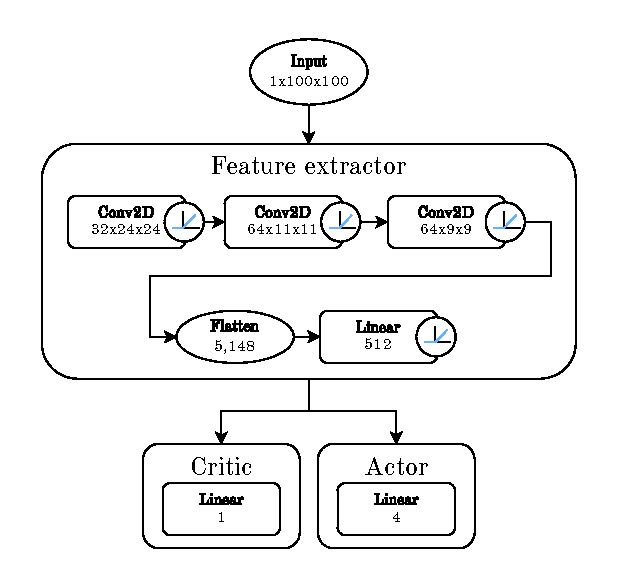
\includegraphics[width=1\linewidth]{diagrams/cnn_arch.pdf}
    \caption{Architecture used by SB3's \texttt{CnnPolicy}.}
    \label{fig:cnn_policy}
\end{figure}

\begin{figure}
    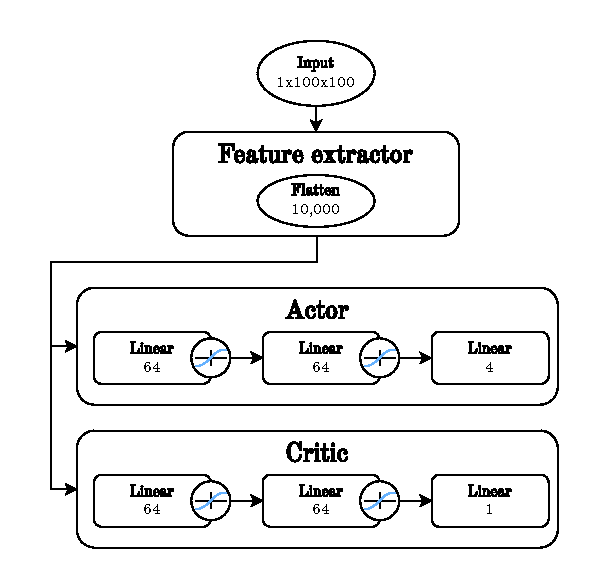
\includegraphics[width=1\linewidth]{diagrams/mlp_arch.pdf}
    \caption{Architecture used by SB3's \texttt{MlpPolicy}.}
    \label{fig:mlp_policy}
\end{figure}

\begin{figure}
    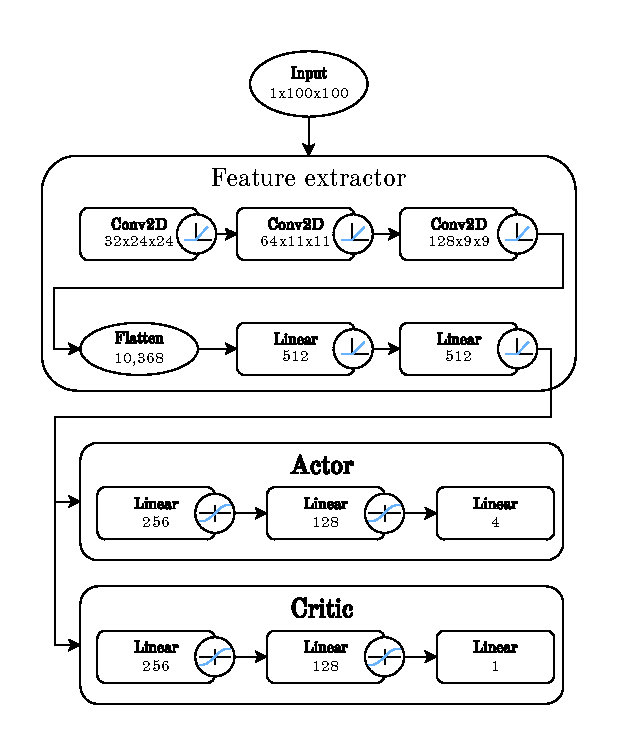
\includegraphics[width=1\linewidth]{diagrams/bigger_net_arch.pdf}
    \caption{Architecture of the network used in Subsection \ref{subsec:arch_change}.}
    \label{fig:bigger_net_policy}
\end{figure}

\begin{figure}
    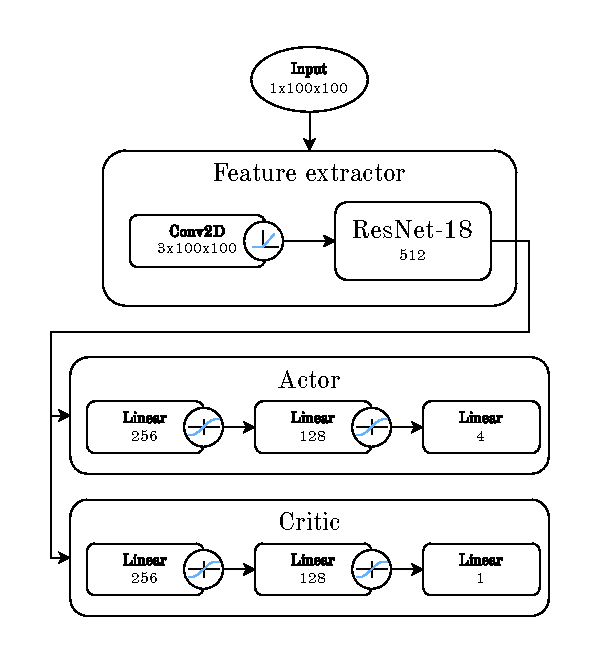
\includegraphics[width=1\linewidth]{diagrams/resnet_arch.pdf}
    \caption{Architecture of the network with a ResNet-18 feature extractor used in Subsection \ref{subsec:resnet}.}
    \label{fig:resnet_arch}
\end{figure}

\begin{figure}
    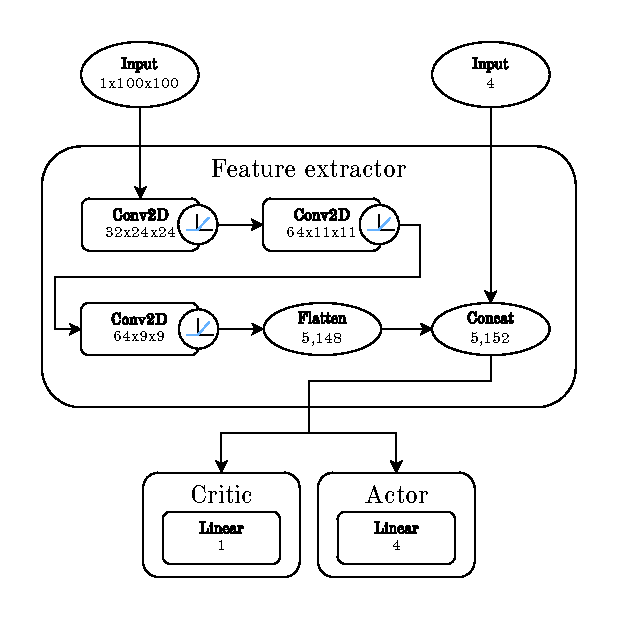
\includegraphics[width=1\linewidth]{diagrams/combined_policy.pdf}
    \caption{Architecture of the multi-input network introduced in Subsection \ref{subsec:eval_metric}.}
    \label{fig:multiinput_arch}
\end{figure}

\chapter{CV detector algorithm}
\label{ap:cv}

This appendix describes in detail the algorithm used in the element detector based on traditional computer vision in Section \ref{sec:trad_cv_detector}. Note that the numerical parameter values mentioned in the text were tuned for images of size $1440\times900$ pixels. For images of a different size, some of them would have to be changed.

\section{Preprocessing}

The algorithm receives a screenshot of a website as input. The first step in the pipeline is preprocessing, which turns the colored image into a binary image that only contains relevant contours.

First, the image is converted from RGB to grayscale. This step is necessary since most image processing algorithms only work on single-channel images. Next, a bilateral filter is applied. Some websites use images or textures as a background, which are then falsely detected as edges. The bilateral filter helps smooth these textures out while not destroying actual edges. This difference can be seen in Figure \ref{fig:bilateral}. I found that $d=21$, $\sigma_s =10$, and $\sigma_r = 50$ worked the best.

\begin{figure}
    \centering
    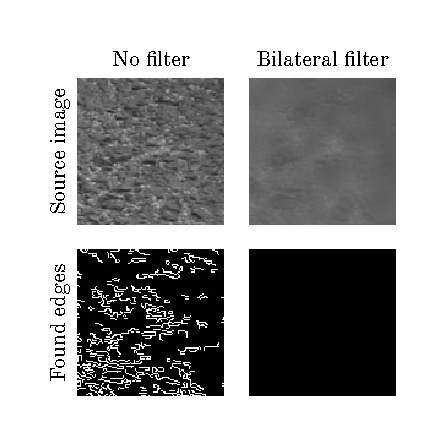
\includegraphics[width=1\linewidth]{diagrams/bilateral.pdf}
    \caption{Comparison of edges detected in an image of a road before and after a bilateral filter is applied. The original image comes from \cite{aydos2020}.}
    \label{fig:bilateral}
\end{figure}

Next, Canny edge detection is used to find edge pixels. I chose Canny in particular since it already implements edge thinning and thresholding. Choosing the thresholds was difficult, since low thresholds lead to noise being detected as edges, while high thresholds could be too strict (for example, filtering out text on a similarly colored background). I got the best results with $t_1=100$ and $t_2=200$.

It would probably be better to do multiple passes of the algorithm with different thresholds for the edge detection (potentially even other steps). Filtering would be more strict with lower thresholds and less strict with higher thresholds. The results of these different passes would then be combined. But since this was supposed to be just a prototype, and finding the right combinations of thresholds and filters would be pretty time-consuming, I decided against it.

Next, the edges are expanded using morphological dilation with a circular kernel. This helps with two problems. First, sometimes the found edges are imperfect and contain holes; the dilation joins them back. Second, it merges letters of a text into a single blob. Deciding whether a contour is a letter or some noise would be complicated without this. This effect is shown in Figure \ref{fig:dilation}.

\begin{figure}
    \centering
    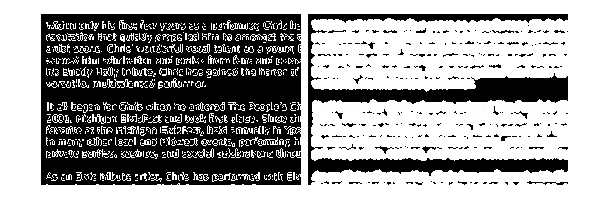
\includegraphics[width=1\linewidth]{diagrams/dilation.pdf}
    \caption{Text after edge detection before and after dilation. The original image comes from \cite{aydos2020}.}
    \label{fig:dilation}
\end{figure}

Unfortunately, the dilation also sometimes joins together two separate elements. I try to somewhat mitigate this by removing one-pixel-wide connections (foreground pixels surrounded by foreground pixels in one direction but not in the other). I detect such pixels using a hit-and-miss transformation and remove them.

After these steps, the image is ready for contour tracing. For this, I use OpenCV's implementation of the Suzuki-Abe algorithm.

\section{Contour filtering}

After the described steps, we now know the locations and points of all contours in the preprocessed image. I first reconstruct the hierarchy of these contours. Note that OpenCV already returns a hierarchy, but it often contains errors. For example, a button with rounded corners frequently has holes in its edges. Because of this, a text inside the button is declared as a sibling contour instead of a child.

To construct the tree, I first create a root contour that runs along the edge of the image and thus contains every other contour. I then sort the found contours in descending order based on the area of their axis-aligned bounding rectangle. Then, for each contour, I check whether its bounding rectangle is mostly within any of the root node's children, in which case I check through its children and repeat recursively. If not, it becomes a new child of the checked node.

Then filtering is done. A contour is eliminated if at least one of the following is true. The filtering results are visible in Figure \ref{fig:filtering}.

\begin{enumerate}
    \item Its bounding rectangle is too small (its height or width is less than 15 pixels, both are under 30 pixels).
    \item Its parent is too small (a contour can only have children if it is at least $100 \times 100$ pixels).
    \item It is too rotated (the angle of the enclosing rectangle with the smallest area is rotated by more than 10 degrees. This rule is not applied to contours of almost square aspect ratio).
    \item It is at least slightly rotated, and the area of its convex hull is notably smaller than that of its bounding rectangle (less than 75 percent).
    \item It is an inside contour (it encloses only background pixels).
\end{enumerate}

\begin{figure}
    \centering
    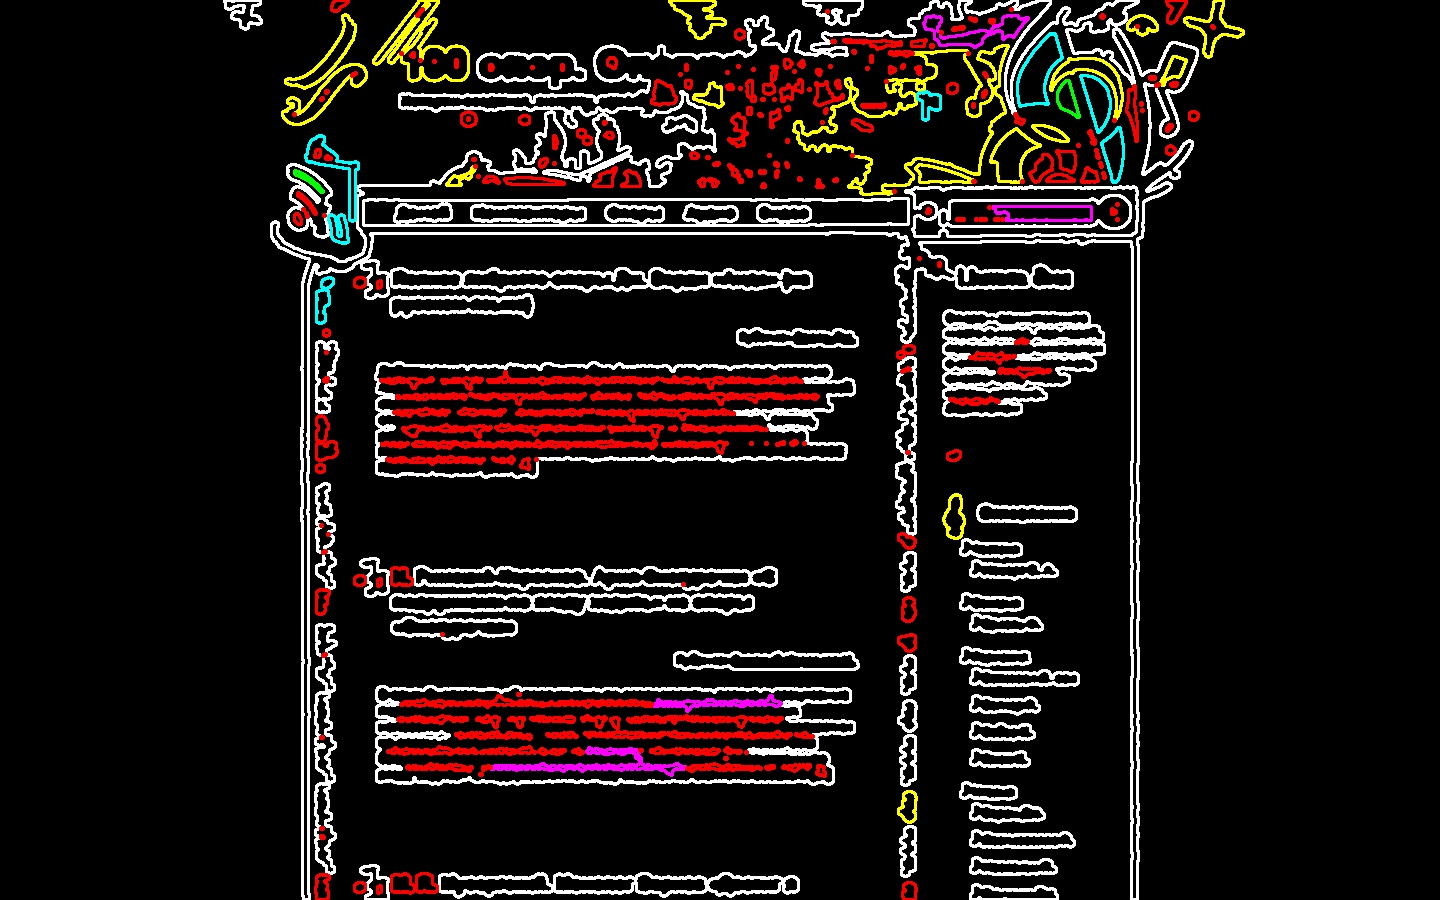
\includegraphics[width=1\linewidth]{diagrams/filter.jpg}
    \caption{The image shows the contour filtering. White contours survived, red contours were too small, green contours' parents were too small, light blue contours were too rotated, yellow contours had a small convex hull, and magenta contours were inside contours. The original image comes from \cite{aydos2020}.}
    \label{fig:filtering}
\end{figure}

Lastly, we merge any two contours whose bounding rectangle intersects, but one is not entirely inside the other. The axis-aligned bounding boxes of these final contours are the algorithm's output.

\chapter{List of digital appendices}

\end{document}
